%% \documentclass[dissertation, copyright, final, justified, numbers, sort&compress]{uothesis}
\documentclass[dissertation, copyright, final, justified, gsmodern]{uothesis}
%% \usepackage[english,UKenglish]{babel}
%% \usepackage{todonotes}
\usepackage{subfig}
\usepackage{caption}
\usepackage{rotating}
\usepackage{makecell}
\usepackage{natbib}
\setcitestyle{round}

%NOTE: I changed this to try and get the better Palatino font
%% \usepackage{amsmath}
\usepackage{mathpazo}
\usepackage{graphicx}
\usepackage{verbatim}
\usepackage{hyperref}
%% \includeonly{cover, abstract, cv, acknowledgements, chapter2}

%Always load this package last
%% \usepackage{cleveref}

% Figure naming macro
\newcommand{\fig}[1]{{\bf Figure \thechapter.#1}}

% Chapter naming macro
\newcommand{\ch}[1]{{\bf Chapter #1}}
%% \newcommand{\Musc}{2}
%% \newcommand{\Thstr}{3}
%% \newcommand{\Amod}{4}
%% \newcommand{\Rev}{5}
\newcommand{\Musc}{II}
\newcommand{\Thstr}{III}
\newcommand{\Amod}{IV}
\newcommand{\Rev}{V}

% Document chapter/section naming
\renewcommand \thechapter{\Roman{chapter}}
%% \renewcommand \thesubsection{\arabic{section}.\arabic{subsection}}

\begin{document}


\covertitle{The Role of Cortical and Subcortical Auditory Pathways in Sound-Driven Behavior}
\abstracttitle{The Role of Cortical and Subcortical Auditory Pathways in Sound-Driven Behavior}
\author{Nicholas Donaldson Ponvert}
\department{Department of Biology}
\narrowdepartment{Department of Biology}
\degreetype{Doctor of Philosophy}

\degreemonth{June}%The month you earn the degree, different than the month you defend
\degreeyear{2019}
\advisor{Santiago Jaramillo}
\chair{Cristopher Niell}
\corememberone{Chris Doe}
\coremembertwo{Michael Posner}
\institutionalrep{Michael Wehr}

\graddean{Janet Woodruff-Borden}

\abstract{
% Making decisions about sound is important for many species
For many species, the ability to use information about sound to guide behavior is important for obtaining rewards such as food, mates, or respite from danger.
% The neural pathways in the brain that associate sounds with actions are not well understood
The neural pathways that associate sounds with actions that will produce reward are not well understood. 
% The auditory pathways through the striatum represent a potential circuit for associating sounds with actions
The striatum, a brain region which receives sound information from the auditory cortex and auditory thalamus, and which can drive behavior via its outputs in the basal ganglia, represents a potential key hub in the pathway between sound and action. 

In this thesis, I investigate the role of striatal circuits in the context of sound-guided behavior, and compare parallel corticostriatal and thalamostriatal pathways that provide auditory information to the striatum.
% 2016astr stuff
In \ch{\Musc}, I inactivate the striatum while animals perform a frequency discrimination task, and find that this manipulation leads to a strong deficit in task performance. 
% 2018thstr stuff
In \ch{\Thstr}, I compare the information about sounds sent to the striatum from the auditory cortex and auditory thalamus.
I find that, while these pathways convey frequency information to the striatum with similar fidelity, they have different representations of temporal modulations in sound amplitude. 
% Amod stuff
In \ch{\Amod} I present a behavioral task that could be used to evaluate the relative contribution of the cortico-striatal and thalamo-striatal pathways to discriminations of different sound features.
%Review stuff
Finally, \ch{\Rev} provides a review of the role of cortical and subcortical pathways in other behavioral contexts, especially in tasks that require rapid flexibility. 

%Need to end with this statement if you're working from papers published or soon to be published.
This dissertation includes previously published co-authored material.
}

\author{Nicholas Donaldson Ponvert}
\school{University of Oregon}
\school{Humboldt State University}
\school{Santa Barbara City College}

\degree{Doctor of Philosophy, Biology, 2019, University of Oregon}
\degree{Bachelor of Science, Biology (Marine), 2014, Humboldt State University}
\degree{Associate of Science, Chemistry, 2012, Santa Barbara City College}

%%There is a known issue if you do not fill in the interests section.  If you want to skip this section, comment out line#526 of uothesis.cls file \cvitem{GRANTS, AWARDS AND HONORS}{\@awards}
\interests{
	\begin{itemize}
        \setlength\itemsep{-0.5em}
		\item Neural basis of behavior
		\item Sensory coding
		\item Circuit mechanisms of learning and memory
		\item High-density extracellular electrophysiology
		\item Calcium imaging
		\item Open-source software
	\end{itemize}
}%Your interests. French movies, long walks on the beach, baking tarts...

\position{Graduate Research Assistant}%Your job while at UO, probably graduate research assistant.
\position{Graduate Teaching Assistant}%Your job while at UO, probably graduate research assistant.

% DONE: Add undergrad awards
\award{Peter O’Day Fellowship graduate student recipient (2017)}
\award{HSU Award for Academic Excellence in CNRS (2014)}
\award{Malcom Oliphant Scholarship Undergraduate Recipient (2013)}
\award{Lilian and Gordon MacGregor Scholarship Recipient (2009, 2011, 2012)}

% DONE: Add publications to CV

\publication{Nicholas D. Ponvert and Santiago Jaramillo (2019). Auditory thalamostriatal and corticostriatal pathways convey complementary information about sound features. \emph{Journal of Neuroscience} 39 (2): 271-280}

\publication{Guo L, Walker WI, Ponvert ND, Penix PL, Jaramillo S (2018) Stable representation of sounds in the posterior striatum during flexible auditory decisions. Nature Communications 9:1534}

\publication{Lan Guo*, Nicholas D. Ponvert* and Santiago Jaramillo (2017). The role of sensory cortex in behavioral flexibility. \emph{Neuroscience} 345: 3-11. *Co-first author}

%% \acknowledge{%Thanks go here.
Thanks to my patient wife Amanda, walk-deprived dog Flora, loving family, and supportive friends for everything I have been able to accomplish.

Extra thanks to everyone in the Jaramillo lab... etc. 

%Leave an extra space before the final curly bracket. At least for me I had some strange problem where the last line became single spaced if I didn't.
}

  %%acknowledgements page optional
\maketitle

\chapter{Introduction}
%Deep thoughts go here.

%% The ability to perceive and react to sounds in the environment is a key adaptation of many species.
% Many levels of sound-driven behavior
From the startled jump that helps an animal avoid a predator, to the complex call-and-response of vocal communication, the ability to associate sounds with rewarding actions is a key adaptation of many species. 
% In some cases, the neural circuits underlying the behavior are well-studied.
% TODO: References regarding brainstem startle response.
% Brainstem circuits: Davis et al. 1982 
% High-level cortical circuits for perception and production of speech:
% Pulvermuller and Fadiga 2010
For some simple sound-action associations, such as the acoustic startle response, the neural pathways supporting the association are well-studied \citep{Davis1982}.
% In other cases, the pathways involved in choosing appropriate actions in response to sounds are not clear.
However, for behaviors that require learning associations between specific sounds and the action that should be taken to get a reward, the neural pathways are not well understood. 

% How to find circuits that are required for a behavior?
One approach for identifying neural pathways that implement certain behaviors is to begin at the ``chunk-of-brain'' level, inactivating or removing certain brain areas to determine which regions are required for task performance.
% Cortex not required for flexible sound-frequency discrimination
In the case of a sound-frequency discrimination task, in which an animal hears a sound and then must make a choice about whether that sound is a ``high'' frequency or a ``low'' frequency, lesion studies have indicated that auditory cortex is not required, pushing the search for the necessary circuitry into subcortical areas \citep{Gimenez2015}.

\section{Cortex is not always required for flexible decision-making about sounds}

Consider the following behavioral task: An animal is required to learn an arbitrary decision boundary between ``high'' and ``low'' sound frequencies, and then correctly categorize sounds as above or below this decision boundary to receive reward.
Then, the decision boundary is varied by the experimenters during the course of a single behavioral session, requiring rapid flexibility on the part of the animal.
Then, once the animal has learned the task, the entire auditory cortex is surgically removed, and the animal is tested to see if it is still able to perform the task.
Taking this approach, \citet{Gimenez2015} found that animals were still able to perform this task to a high degree of accuracy after nearly-complete lesion of auditory cortex.
However, lesions of auditory thalamus completely impaired the ability of animals to perform the task. 
These results suggest that a subcortical output pathway of the auditory thalamus is sufficient to mediate this task.

The auditory thalamus, while often viewed as a stop along the way for information about sounds traveling from the periphery to the auditory cortex, has several subcortical outputs as well.
% DONE: Citations for 3 main subcortical outputs of auditory thalamus.
The main subcortical projection targets for auditory thalamus neurons are the thalamic reticular nucleus, the amygdala, and the striatum \citep{Pinault2004, Bartlett2013}.
Of these targets, the amygdala and the striatum are the most likely candidates for forming associations between sounds and actions.
% TODO: Citations for thalamic reticular nucleus
The thalamic reticular nucleus is composed primarily of inhibitory neurons that provide a recurrent inhibitory circuit back onto neurons in the auditory thalamus \citep{Pinault2004}. 
% DONE: Citations for amygdala fear learning to auditory stimuli.
The amygdala has been extensively studied in the context of fear conditioning, and much is known about how amygdalar circuits change during learning to associate auditory stimuli with noxious stimuli and promote fear responses \citep{Romanski1992, Rogan1997, Doron1999, Ledoux2000}. 
%
While these neurons have also been shown to encode both positive and negative valence of sensory cues \citep{Tye2008}, they seem to play only a minimal role in forming associations between stimuli and actions that will bring reward \citep{Baxter2002}.

% DONE: Citations for striatum in context of Parkinson's
The striatum, regions of which have been studied in the context of motor initiation \citep{Graybiel1994, Hikosaka2000a} and in disorders such as Parkinson's disease \citep{Huot2007, Kravitz2010, Parker2016}, has also been shown to play a key role in reward-related learning \citep{Wickens2003, Balleine2007}.
%% Regions of the striatum, in contrast, have been shown to play a key role in reward-related learning 
% DONE: Dopaminergic innervation citations. 
In addition to receiving information about sound from the auditory thalamus and the auditory cortex, it is also the target of extensive dopaminergic innervation from the substantia nigra pars compacta \citep{Menegas2015, Menegas2017}
% DONE: Basal ganglia citations here.
Additionally, the striatum is a primary input to the basal ganglia, which are involved in the control of voluntary movements \citep{Smith1998, Kravitz2010}.
The striatum is therefore ideally situated to act as a key hub in associating sounds with actions that bring rewards.

\section{The striatum and decision making}
% The striatum, historical association with reward and motor function
Recent studies focusing on the pathway between auditory cortex and the striatum have pointed to a role for this pathway in associating sounds with rewarded actions.
% Petr's paper
First, manipulation of the corticostriatal pathway produces predictable biases in a frequency-discrimination task \citep{Znamenskiy2013}.
% Q's paper
Second, the synaptic efficacy between auditory cortical neurons and their MSN targets changes as animals learn a frequency-discrimination task in a way that could support the learned association \citep{Xiong2015}.
%%%%%%%% CHAPTER 2 PLUG HERE %%%%%%%%%%%%%
Additionally, results of experiments in \ch{\Musc}, previously published as part of \citet{Guo2018}, establish a critical role for posterior striatal circuits in the performance of a sound-frequency discrimination task. 
% DONE: Overview and Zador model
Taken together, these studies point towards a potential model for formation and maintenance of sound-action associations, in which learning strengthens connections between auditory cortex neurons that represent the relevant stimulus and striatal neurons that can promote the rewarded choice.
%
However, this model is inconsistent with the fact that animals can readily perform behaviors based on learned sound-action associations after nearly complete lesions of auditory cortex.
%
This evidence suggests a role for the thalamostriatal pathway as well.

\section{Parallel cortical and subcortical pathways}

% DONE: Little is known? Or was known?
Few studies have investigated the relationship between the parallel corticostriatal and thalamostriatal pathways, and so the relative contribution of these two pathways to sound-action association is still not well established.
% Role of parallel cortical and subcortical pathways in other systems (like fear).
One hypothesis is that the thalamostriatal pathway sends redundant information about sound, facilitating discrimination of simple, tonal stimuli even after extensive cortical lesion.
% Instead we think they send complementary info
% DONE: Do I want to put this more specific hypothesis in the main intro?
We hypothesized instead that information about sounds sent by auditory thalamostriatal and corticostriatal neurons is complementary, with specific sound features differentially encoded by these two pathways.
%%%%%%%% CHAPTER 3 PLUG HERE %%%%%%%%%%%%%
In \ch{\Thstr}, previously published as \citet{Ponvert2019}, we perform pathway-specific electrophysiology to investigate and compare the sound features encoded by these parallel pathways.
%
We find that the two pathways represent some features of sounds, like sound frequency, in a similar way.
%
For other sound features, such as the rate of temporal modulations in amplitude, the two pathways appear to convey complementary stimulus representations to the striatum.
%
These findings suggest that the two pathways may be differentially recruited depending on the relevant features in a task. 

\section{Are the differences in information sent by the two pathways behaviorally relevant?}
% DONE: When would you need the different kind of features? 
% Pull stuff from the review here, etc.
Lesions of auditory cortex have been found to have different effects on performance of behaviors relying on sound-action associations depending on the specific auditory stimulus feature to which the action must be associated.
%
For instance, while rats with bilateral lesions of auditory cortex were able to perform discriminations of sound frequency \citep{Gimenez2015}, a different study found that lesions of AC in gerbils trained to discriminate between fast and slow modulations in sound amplitude strongly impaired task performance \citep{Deutscher2006}.
%
This suggests that the representation of some stimulus features, such as AM rate, that are provided by the cortex may be necessary for successful discrimination of that feature.
%
In contrast, discrimination of sound frequency may be possible with subcortical representations of this feature alone.
%
We hypothesized that inactivation of auditory cortex would have a stronger effect on discrimination of AM rate than on discrimination of sound frequency.
%
To test this hypothesis, we trained animals to perform discriminations of both sound frequency and AM rate within the same behavioral session, allowing us to test the effect of the same manipulation of AC on both discriminations.
%%%%%%%% CHAPTER 4 PLUG HERE %%%%%%%%%%%%%
% DONE: Finish this task
In \ch{\Amod} I present this task and show that animals can be trained to perform the two discriminations during the same behavioral session with a high degree of accuracy.
%

%%%%%%%% CHAPTER 5 PLUG HERE %%%%%%%%%%%%%
% DONE: This sounds like the abstract so far. 
Lastly, in \ch{\Rev} (previously published as \citet{Guo2017}) we expand to discuss the role of sensory cortex in behavioral flexibility more broadly.
%
We propose a taxonomy of flexible behaviors, and review the literature that suggests that some types of task/stimulus combinations are dependent on sensory cortex, while others can be mediated by subcortical pathways.
%
% BOOM!
Overall, \ch{\Thstr} provides a framework for studying the convergence of cortical and thalamic information onto the striatum, \ch{\Amod} provides a behavioral task for comparing the relative dependence of discriminations of different stimulus features on information from a specific pathway, and \ch{\Rev} provides a starting point for investigating the relative contributions of cortical and subcortical pathways to flexible behaviors across different sensory modalities. 

%% \section{What does it mean to understand how the brain accomplishes a task?}
%% There are different levels of understanding of a system.
%% We want to understand: (1) What regions of the brain are critical for performance of sound-guided decision making tasks? (2) What information about sound reaches this region? (3) How does the region choose appropriate actions in response to a sound? (4) What pre-processing of sound information is necessary for the region to form associations between sound features and behaviors that will bring reward? 
 % Introduction
% Figures in this chapter
\newcommand{\Muscimol}{1}
\newcommand{\MuscimolDiagram}{\Muscimol A}
\newcommand{\MuscimolExample}{\Muscimol B}
\newcommand{\MuscimolSummary}{\Muscimol C}
\newcommand{\MuscimolSites}{2}
\newcommand{\FluorescentMuscimol}{3}
\newcommand{\MuscimolMovement}{4}
\newcommand{\MuscimolNumTrials}{\MuscimolMovement A}
\newcommand{\MuscimolCoutTime}{\MuscimolMovement B}
\newcommand{\MuscimolSideInTime}{\MuscimolMovement C}

\chapter{Striatal circuits are involved in sound frequency discrimination.}

\section{Author contributions}
\noindent Originally published as part of: Lan Guo, William I Walker, Nicholas D Ponvert, Phoebe L Penix, and Santiago Jaramillo, 2018.  Stable representation of sounds in the posterior striatum during flexible auditory decisions. \textit{Nature Communications} 9 (1534).
%
Santaigo Jaramillo provided mentorship for all aspects of the study. Nicholas D Ponvert performed all experiments included in this dissertation. Lan Guo, Nicholas D Ponvert, and Santiago Jaramillo wrote the sections of the paper pertaining to the results of the behavioral experiments included in this dissertation. 

\section{Introduction}
% DONE: This section mostly from the paper. I'm leaving it.
In the mammalian brain, the dorsal striatum links neural signals from the cerebral cortex to circuits in the basal ganglia to mediate action selection. Electrophysiological and inactivation studies have identified two regions within the dorsal striatum which play distinct roles in decision making: the dorsomedial striatum (DMS) involved in flexible goal-oriented behavior, and the dorsolateral striatum (DLS) which mediates habitual actions \citep{Yin2006, Balleine2009, Devan2011}.
%
Recent anatomical characterization of the excitatory input from cortex and thalamus onto the striatum suggests that the organization of the dorsal striatum goes beyond the DMS and DLS divide \citep{Hunnicutt2016}.
%
This characterization in rodents showed that the posterior portion of the striatum receives a combination of sensory inputs that sets it apart from other regions.
%
Similarly, an evaluation of reward-related signals of the dopaminergic input along the anterior-posterior axis of the striatum provides further evidence that the posterior tail of the striatum forms a circuit distinct from the anterior dorsal striatum, which includes the classically studied DMS and DLS regions \citep{Menegas2015, Menegas2017}.
%
It is not clear, however, whether the function of this posterior region is qualitatively different from the previously characterized striatal subregions.
%
Here, we evaluate the role of neurons in the posterior tail of the striatum during sensory-driven decisions in mice.

The posterior tail of the dorsal striatum in rodents (referred to hereafter as posterior striatum) receives direct neuronal projections from the auditory thalamus (ATh) and the auditory cortex (AC), as well as midbrain dopaminergic signals \citep{Menegas2015, Hunnicutt2016}.
%
Because of these anatomical features, this region is sometimes referred to as the auditory striatum \citep{Znamenskiy2013}.
%
Given this convergence of sensory and reward-related signals, and prompted by the role of other dorsal striatal regions, we hypothesized that the posterior striatum drives rewarded actions according to acoustic cues.

In this chapter, we train animals to perform a simple sound-frequency discrimination task, and then perform reversible inactivation of the posterior striatum to determine whether the region is necessary for task performance.
%
We observe strong deficits in task performance during sessions in which striatum was inactivated, supporting the hypothesis that this region plays a key role in tasks that require sound-action association.

\section{Methods}

\subsection{Animal subjects}
5 adult male wild-type mice (C57/BL6J) were used in this study. Mice had ad libitum access to food, but water was restricted. Free water was provided on days with no experimental sessions. All procedures were carried out in accordance with National Institutes of Health standards and were approved by the University of Oregon Institutional Animal Care and Use Committee.

\subsection{Behavioral task}
Behavioral data was collected using the taskontrol platform (\url{www.github.com/sjara/taskontrol}) developed in our laboratory using the Python programming language (\url{www.python.org}). Mice initiated each trial by poking their noses into the center port of a three-port behavior chamber. After a silent delay of random duration (150-250 ms, uniformly distributed), a narrow-band sound (chord) was presented for 100 ms. Animals were required to stay in the center port until the end of the sound and then chose one of the two side ports for reward (2 ul of water) according to the frequency of the sound (low-frequency: left port; high-frequency: right port). If animals withdrew before the end of the stimulus, the trial was aborted and ignored in the analysis. Stimuli were chords composed of 12 simultaneous pure tones logarithmically spaced in the range f/1.2 to 1.2f for a given center frequency f. Within a behavioral session, we used 6 or 8 distinct center frequencies. The intensity of all sound components was set to the same value between 30-50 dB-SPL (changing from one trial to the next) during the initial training, but fixed during testing at 50 dB-SPL. Each behavioral session lasted 60 to 90 minutes.

\subsection{Muscimol inactivation}
Bilateral craniotomies were performed under stereotactic surgery over the posterior striatum (1.7 mm posterior to bregma, 3.55 mm lateral from midline) of mice trained in the two-alternative choice sound discrimination task. Headbars were implanted to allow for head-fixation. Each craniotomy was protected with a plastic ring and filled with silicon elastomer (Sylgard 170, Dow Corning). Animals were allowed to recover for at least 3 days before resuming behavioral training. Following recovery, implanted animals were trained on the sound discrimination task until they reached their pre-surgery performance level before beginning muscimol inactivation.

For intracranial injection, we used glass pipettes (5 ul Disposable Micropipettes, VWR) pulled and trimmed to an inner diameter of 15-20 micrometers at the tip. Animals were head-fixed and allowed to run on a wheel during the injection. Craniotomies were exposed by removing the silicon elastomer covering, and a glass pipette filled with reagent (either muscimol or saline) was lowered into the brain to a depth of 3.1mm from brain surface using a micromanipulator. A volume of 45 nl of muscimol (0.25 mg ml$^{-1}$, final dose of 11.25 ng per hemisphere) was injected under air pressure in each hemisphere at a rate of 90 nl min$^{-1}$.
%
Given the relationship between concentration and diffusion distance (from Fick's law) and previous reports of muscimol effects on neuronal activity \citep{Edeline2002}, we expect that by the first 10 minutes of the behavioral session, the effects of muscimol (50\% reduction in firing or more) will be confined to a volume smaller than 1 mm in diameter centered at the injection site. This volume matches well the extent of the posterior tail of the striatum (approx. 1 mm A-P, 0.6 mm M-L, 1.5 mm D-V) that receives auditory inputs \citep{Hunnicutt2016}.
%
The pipette was left in place for 60 seconds following the injection, then raised 0.5mm and left in place for another 60 seconds before being removed. Injection in the second hemisphere was always completed within 10 minutes of the first injection. The craniotomies were then protected with a new silicon elastomer cap, and the mouse was placed back into its home cage for 30 minutes before starting the behavior session. After collection of 4 saline sessions and 4 muscimol sessions, 45 nl of fluorescent dye (DiI, Thermo Fisher Scientific) was injected at the same injection coordinates. Animals were then perfused transcardially with 5\% paraformaldehyde, and brains were extracted and postfixed for 12-24 hours. Brains were then sliced (100 um) and imaged to verify the location of fluorescent dye injection.

Fluorescent muscimol (Muscimol, BODIPY TMR-X Conjugate, Thermo Fisher Scientific) was dissolved in phosphate-buffered saline to a final concentration of 0.5 mg ml$^{-1}$. We followed the same protocol for intracranial injection as for muscimol. The injection volume was 360 nl per hemisphere (final dose of 180 ng per hemisphere) to account for the larger molecular weight and reduced spread of fluorescent muscimol. As with muscimol injections, animals rested for 30 minutes before starting the behavior session. Animals were euthanized and transcardially perfused with 5\% paraformaldehyde within 1 hour of finishing behavioral testing. Brains were extracted and postfixed overnight, and sliced (100 um) to quantify spread of fluorescent muscimol.

\subsection{Analysis of behavioral data}

Psychometric curve fitting was performed via constrained maximum likelihood to estimate the parameters of a logistic sigmoid function (\url{http://psignifit.sourceforge.net}). Statistical comparisons were performed using non-parametric statistical tests with no assumption of normality. 

\section{Results}

%%%%% Section - Change in overall performance %%%%%%%%
To test whether the activity of posterior striatal neurons was required when performing the sound-discrimination task, we quantified task performance during bilateral reversible inactivation of  these neurons (\fig{\Muscimol}, \fig{\MuscimolSites}).
%
Injection of muscimol (a GABA-A receptor agonist) in the posterior striatum resulted in a consistent decrease in task performance compared to injection of saline as control (\fig{\MuscimolExample}).
%
The effect was observed in all mice tested (\fig{\MuscimolSummary}, $p<0.05$ for each mouse, Wilcoxon rank-sum test), and consisted of a flattening of the psychometric curve.
%
Repeated injections did not alter task performance across the saline sessions tested ($r=-0.24$, $p=0.75$, linear regression of accuracy on sessions).
%
These results were replicated using fluorescent muscimol to confirm that inactivation restricted to the posterior striatum affected task performance (\fig{\FluorescentMuscimol}).

%%%%% Section - Movement effects %%%%%%%%

%
As a result of muscimol inactivation, mice displayed slower withdrawals from the center port on average ($p<0.05$ for four out of five mice, Wilcoxon rank-sum test, \fig{\MuscimolCoutTime}).
%
A change in movement speed from the center port to the reward ports was observed in only one out of five mice ($p<0.05$, Wilcoxon rank-sum test, \fig{\MuscimolSideInTime}).
%
Even though animals displayed motor impairments during muscimol inactivation, they still performed hundreds of trials during each session (480$\pm$146 muscimol \emph{vs.} 733$\pm$86 saline, \fig{\MuscimolNumTrials}, $p<0.05$ for three out of five mice, Wilcoxon rank-sum test).
%
During inactivation sessions, some animals used a strategy in which they chose a reward port at random, while other animals displayed a strong bias to one side.
%
Both of these strategies resulted in an average performance close to chance level for the binary choice.

% TODO: I should use a figure that has a better description of the task here.
\begin{figure}[!p]
  \begin{center}
    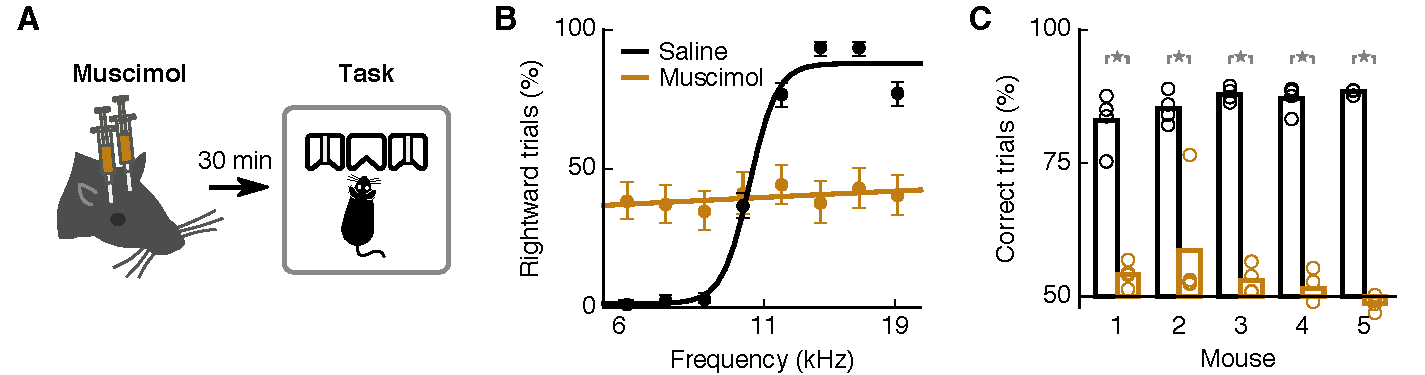
\includegraphics[width=5in]{figures/chapter2/Fig3_muscimol_inactivation}% 
  \end{center}
  \caption{Inactivation of posterior striatum impairs task performance.}{\textbf{(A)} Animals received bilateral injections of muscimol in the posterior
  striatum 30 minutes prior to starting the sound-frequency discrimination task. \textbf{(B)} During muscimol injection sessions (brown), animals performed significantly worse in the discrimination task than on days with control injections of saline (black). \textbf{(C)} Muscimol injection (brown) reduced performance to near chance level compared with saline injection (black) in all animals tested.}
\end{figure}


\begin{figure}[!p]
  \begin{center}
    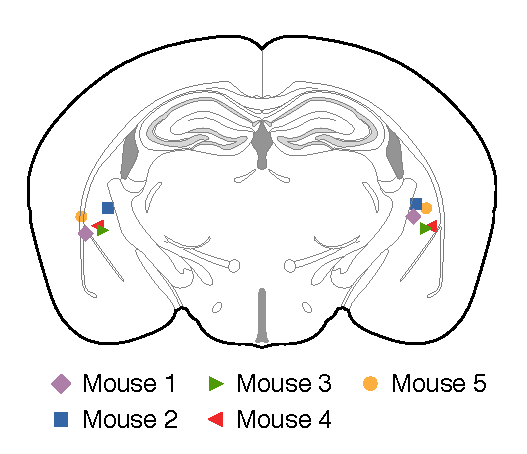
\includegraphics[width=3in]{figures/chapter2/SFig3_muscimol_injection_sites}% 
  \end{center}
  \caption{Location of muscimol injection sites.}{Injection sites were well-clustered and primarily contained to the posterior striatum.}
\end{figure}


\begin{figure}[!p]
  \begin{center}
    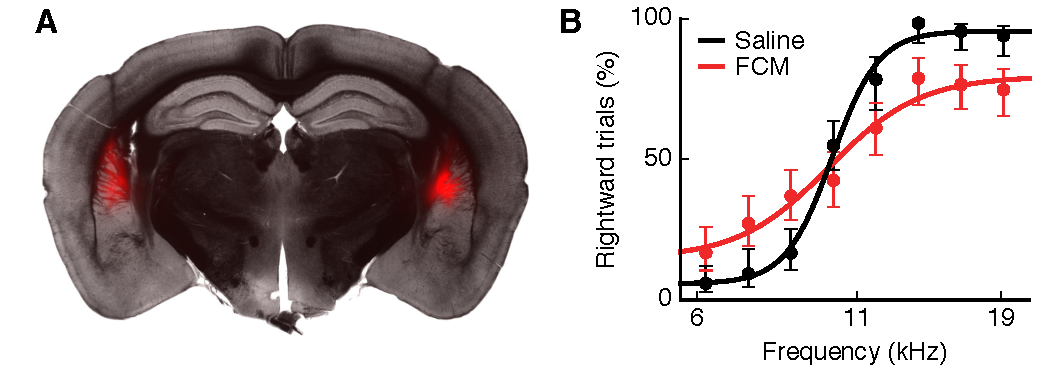
\includegraphics[width=5in]{figures/chapter2/SFig4_muscimol_inactivation_fluorescent}% 
  \end{center}
  \caption{Fluorescent muscimol well-restricted to posterior striatum causes reduction in task performance.}{\textbf{(A)} Muscimol conjugated with the fluorescent marker BODIPY was injected in the posterior striatum. In a histological section taken immediately after the behavior session, the extent of the muscimol injection is visible. \textbf{(B)} Injection of fluorescent muscimol affects discrimination performance in the frequency discriminaton task.}
\end{figure}



\begin{figure}[!p]
  \begin{center}
    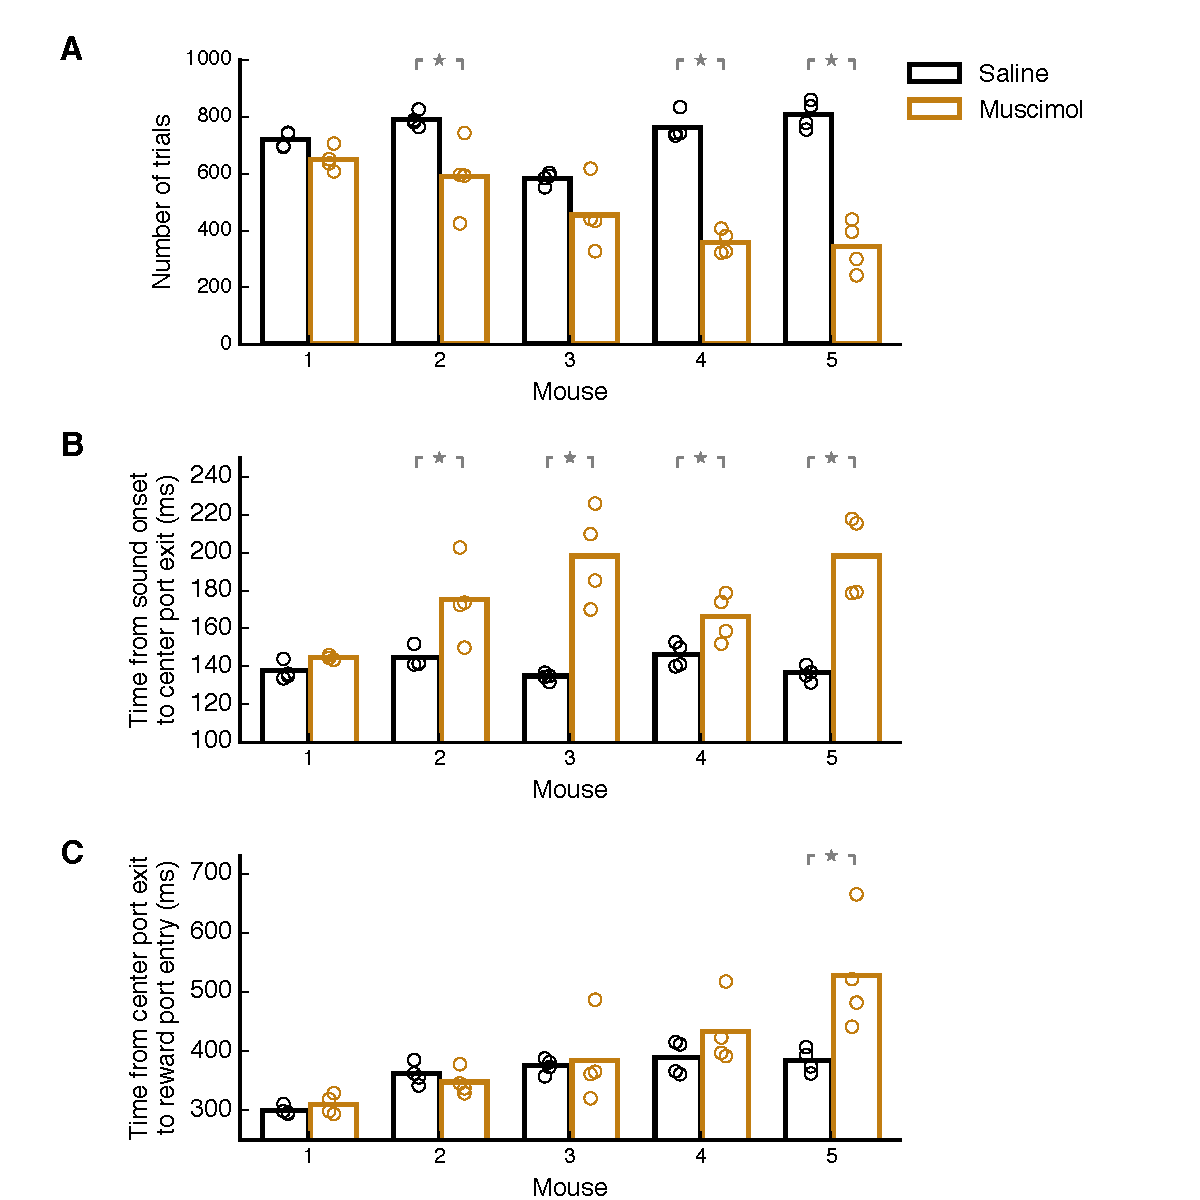
\includegraphics[width=5in]{figures/chapter2/SFig5_muscimol_inactivation_numtrials}% 
  \end{center}
  \caption{Inactivation of posterior striatum causes minimal motor impairment.}{\textbf{(A)} Three out of five animals tested performed significantly fewer trials in behavior sessions following muscimol injection (brown) compared to saline injection (black). \textbf{(B)} The delay between when the animal heard the sound and when it withdrew from the center port was significantly longer after muscimol injection for 4 out of 5 animals. \textbf{(C)} Only 1 out of 5 animals took longer to reach the side port after withdrawing from the center port.}
\end{figure}

\section{Discussion}

% This stuff is consistent with Zador lab stuff.
Recent studies of the corticostriatal pathway have proposed a model in which learning increases the efficacy of the synapses between neurons in auditory cortex that represent an auditory stimulus and neurons in the striatum that promote the action the animal should take after hearing that sound in order to get a reward \citep{Znamenskiy2013, Xiong2015}.
%
% DONE: A little more detail about the rest of the results in the paper here, but not much.
While the inactivation experiments described in this chapter are consistent with this model,  it does not fully account for other results described in \citet{Guo2018}.
%
For instance, in experiments where the categorization boundary was changed during the course of a single behavior session, requiring animals to switch the action associated with a particular stimulus, the sound responses of the large majority of posterior striatal neurons remains stable. 
%
If the sound-action association was encoded in the strength of the synapses between auditory areas and the posterior striatum, then the sound-evoked responses of posterior striatal neurons would be expected to change when the animal adapts to a new stimulus-action association.
%
Instead, the results of this study were more consistent with posterior striatal neurons providing information about the identity of the auditory stimulus, without considerable modulation by the subsequent choice. 

Our inactivation experiments demonstrate that silencing auditory striatal neurons has a drastic effect on a task that requires sound-driven decisions.
%
One interpretation of these results states that these neurons belong to a unique pathway required for successful performance of the frequency discrimination task we study.
%
Alternatively, these neurons could form one of several parallel pathways linking sensation to action, and reversible inactivation yields strong effects on behavior by altering the dynamics of downstream circuits.
%
Our experiments cannot distinguish between these possibilities, yet, provide strong support for a role of these striatal neurons in sensory-driven decisions.

In contrast with stimulation of anterior striatal regions, optogenetic stimulation of posterior striatal neurons did not elicit movements. 
%
On the other hand, we did find that chemical inactivation of the posterior striatum resulted in some motor effects.
%
However, motor impairment alone does not account for the performance deficits
observed during muscimol injection.
%
% DONE: Verify this number and the one below. 
In fact, only one animal tested took significantly longer to reach the side
reward port after withdrawing from the center port.
%
% DONE: So what?
Four out of five animals tested displayed a longer latency to withdraw from the center port
after hearing the sound during muscimol sessions, suggesting an impairment in sensory processing, decision making, or motor initiation rather than a direct impairment of motor function. 
%
% DONE: Come back to this sentence
Additionally, the reduced trial number observed during muscimol sessions in 3 out of 5 animals tested could also be the result of animals becoming frustrated and disengaging from the task due to a reduction in the number of earned rewards.

\section{Link to Chapter III}

In this chapter we found that the posterior striatum is a key region for performing a sound frequency-categorization task.
%
Previous studies had suggested a role for the pathway between auditory cortex and the posterior striatum in performance of a similar task, consistent with our results here \citep{Znamenskiy2013, Xiong2015}.
%
However, animal have also been shown to be capable of performing similar frequency-categorization tasks after nearly-complete removal of auditory cortex.
%
We therefore investigated the other source of auditory input to the posterior striatum, the thalamostriatal pathway. 
%
We compared the auditory information sent by the thalamostriatal pathway to that sent by the corticostriatal pathway to determine whether these pathways represent features of sound in a redundant or complementary way. 

 % Muscimol inactivation
%Figures in this chapter
\newcommand{\Anatomy}{1}
\newcommand{\AnatomyInjection}{\Anatomy A}
\newcommand{\AnatomyThalExample}{\Anatomy B}
\newcommand{\AnatomyThalSummary}{\Anatomy C}
\newcommand{\AnatomyThalamus}{\Anatomy B, C}
\newcommand{\AnatomyACExample}{\Anatomy D}
\newcommand{\AnatomyACSummary}{\Anatomy E}
\newcommand{\AnatomyAC}{\Anatomy D, E}

\newcommand{\Method}{2}
\newcommand{\MethodDiagram}{\Method A}
\newcommand{\MethodDirectCell}{\Method B}
\newcommand{\MethodDirectCellAndNBQXPop}{\Method B, F}
\newcommand{\MethodIndirectNoFollow}{\Method C}
\newcommand{\MethodLongLatency}{\Method C, D}
\newcommand{\MethodIndirectFollows}{\Method D}
\newcommand{\MethodSoundCharPop}{\Method E}

\newcommand{\NoiseLaser}{3}
\newcommand{\NoiseLaserThalDiagram}{\NoiseLaser A}
\newcommand{\NoiseLaserThalExample}{\NoiseLaser B}
\newcommand{\NoiseLaserThalLocations}{\NoiseLaser C}
\newcommand{\NoiseLaserACDiagram}{\NoiseLaser D}
\newcommand{\NoiseLaserACExample}{\NoiseLaser E}
\newcommand{\NoiseLaserACLocations}{\NoiseLaser F}
\newcommand{\NoiseLaserDiagrams}{\NoiseLaser A, D}

\newcommand{\Frequency}{4}
\newcommand{\FrequencyThalExample}{\Frequency A}
\newcommand{\FrequencyACExample}{\Frequency B}
\newcommand{\FrequencyBW}{\Frequency C}
\newcommand{\FrequencyThreshold}{\Frequency D}
\newcommand{\FrequencyLatency}{\Frequency E}
\newcommand{\FrequencyOnsetivity}{\Frequency F}
\newcommand{\FrequencyMonotonicity}{\Frequency G}

\newcommand{\AM}{5}
\newcommand{\AMThalExamples}{\AM A, B}
\newcommand{\AMACExamples}{\AM E, F}
\newcommand{\AMPies}{\AM C}
\newcommand{\AMSync}{\AM D}
\newcommand{\AMRateDiscrim}{\AM G}
\newcommand{\AMPhaseDiscrim}{\AM H}

\chapter{Thalamostriatal and corticostriatal pathways convey complementary information about sound features}

\section{Author contributions}
\noindent Originally published as: Nicholas D Ponvert and Santiago Jaramillo, 2019. Thalamostriatal and corticostriatal pathways convey complementary information about sound features. \textit{Journal of Neuroscience} 39 (2): 271-280. 
%
Santaigo Jaramillo provided mentorship for all aspects of the study. Nicholas D Ponvert performed all experiments included in this dissertation. Nicholas D Ponvert and Santiago Jaramillo wrote the sections of the paper. 

\section{Introduction}
Recent experiments have begun to establish the role of the neural pathway from auditory cortex to the striatum during decision making.
%
Activation of striatal-projecting auditory cortical neurons during a sound discrimination task biases decision making in a frequency-specific way \citep{Znamenskiy2013}, and the synaptic strength between auditory cortical neurons and striatal neurons changes during acquisition of a sound-discrimination task in a way that could support the learned sound-action association \citep{Xiong2015}. 
%
In contrast, the role of the parallel auditory pathway from the thalamus to the striatum is not known.
%
One hypothesis is that this thalamostriatal pathway sends redundant information about sounds, facilitating discrimination of simple, tonal stimuli even after extensive cortical lesions \citep{Gimenez2015, Guo2017}.
%
We hypothesized instead that information about sounds sent by auditory thalamostriatal and corticostriatal neurons is complementary, with specific sound features differentially encoded by these two pathways.

To test this hypothesis, we used an optogenetic approach in awake mice to identify responses from striatal-projecting neurons in auditory thalamus and auditory cortex during extracellular recordings, while presenting sounds of various frequencies and temporal modulations.
%
We found that the two pathways convey information about sound frequency to the striatum with similar fidelity.
%
In contrast, thalamostriatal neurons provide more information about the timing (phase) of amplitude modulated sounds than corticostriatal neurons.
Moreover, the number of evoked spikes in corticostriatal neurons encodes amplitude modulation (AM) rate more accurately than that of thalamostriatal cells. 
%
Downstream circuits capable of linearly decoding spike counts would therefore be better able to discriminate AM rates using corticostriatal inputs compared to thalamostriatal inputs.
%
These findings shed light on the relative contributions of the thalamostriatal and corticostriatal pathways to sound-driven decision making.

\section{Methods}
\subsection{Animals}
%
We used 9 transgenic mice in this study. 
%
Three male and two female transgenic mice expressing Channelrhodopsin-2 in a \textit{Cre} recombinase-dependent manner (LSL-ChR2 mice, JAX number 012569) were used for electrophysiological recordings. 
%
One male LSL-ChR2 mouse was used for NBQX validation of photoidentification methods.
%
Three male mice expressing the fluorescent protein tdTomato in a \textit{Cre} recombinase-dependent manner (Ai14 mice, JAX number 007914) were used in anatomical experiments. 
%
Mice had \textit{ad libitum} access to food and water. Mice used for electrophysiology were between 8 and 14 weeks old at the time of viral injection. 
%
Mice used for anatomy were between 12 and 31 weeks old at the time of viral injection. 
%
All procedures were carried out in accordance with National Institutes of Health Standards and were approved by the University of Oregon Institutional Animal Care and Use Committee.


\subsection{Viral injections}
%
Animals were anesthetized with 2.5\% isoflurane and placed on a stereotaxic surgical apparatus. 
%
The skull was exposed, and a 0.5 mm burr-hole was drilled at the injection coordinates over posterior striatum (A-P: -1.7 mm from bregma, M-L: 3.5 mm right of midline, D-V: -2.75 mm from pia). 
%
A pulled glass pipette (5 $\mu$l, VWR) with a final tip diameter of 15-20 $\mu$m was backfilled with a strain of Canine Adenovirus Type 2 engineered to deliver the gene for \textit{Cre} recombinase (CAV2-Cre, Montpellier Vector Platform) and then lowered into the brain to the injection depth.
%
A 45 nL bolus of CAV2-Cre was then injected manually under air pressure at a rate of 90 nL/min.
%
Two minutes after the injection was complete, the glass pipette was withdrawn 250 $\mu$m.
%
After 1 more minute, the pipette was withdrawn an additional 500 $\mu$m. 
%
After a final 1 minute delay, the pipette was removed and the skin was closed with cyanoacrylate tissue adhesive (VetBond, 3M). 
%
A minimum of 20 days was allowed for expression of the virus before further procedures were carried out. 

\subsection{Electrophysiology and photoidentification of striatal-projecting neurons}
%
In preparation for head-fixed awake electrophysiological recordings, a headbar was attached to the skull of animals under anesthesia.
%
Animals were anesthetized with 2.5\% isoflurane and placed on a stereotaxic surgical apparatus. 
%
The scalp was removed, the headbar was fitted to the skull, and craniotomies were made posterior to the headbar over the coordinates for auditory thalamus (AP: -3.2 mm from bregma, ML: 2.0 mm right of midline) and auditory cortex (AP: -2.8 mm from bregma, ML: 4.4 mm right of midline), ipsilateral to the virus injection.
%
The dura mater was removed. 
%
A plastic well was attached to the skull over each craniotomy and filled with a silicone elastomer (Sylgard 170, Dow-Corning) to protect the brain surface. 
%
Animals were allowed to recover for a minimum of 4 days before beginning electrophysiology experiments.

On each recording session, animals were head-fixed and allowed to run on a wheel inside a single-walled sound-isolation box (IAC-Acoustics). 
%
The silicone plug was removed from the well, and electrodes were inserted through the well into the brain. 
%
All recordings were performed with 4-shank, 32-channel silicon probes with electrodes arrayed in tetrodes (A4x2-tet-5mm-150-200-121, NeuroNexus). 
%
Data were collected using an RHD2000 acquisition system (Intan Technologies) and the OpenEphys software (\url{http://www.open-ephys.org/}).
%
Shanks were marked with a fluorescent dye (DiI: Cat \#V22885, or DiD: Cat \#V22887, Thermo-Fisher Scientific) before penetration to facilitate post-mortem imaging of electrode tracts. 
%
Silicon probes were fitted with a 50 $\mu$m diameter optical fiber (Polymicro Technologies) placed between the two middle shanks and terminating 450 $\mu$m from the tip of the probe (200 $\mu$m above the tetrode farthest from the tip). 
%
This optical fiber was used to deliver 445 nm laser light (1.5 mW at the fiber tip).

To find striatal-projecting neurons, we presented 100 ms pulses of light and 100 ms bursts of 60 dB SPL white noise. 
%
We continued recording only if we found both light-evoked and sound-evoked responses. 
%
We next presented trains of 10 ms light pulses at 5 Hz to distinguish between neurons expressing ChR2 and those indirectly activated via synaptic input from ChR2-positive neurons \citep{Lima2009}, see ``Automatic selection of ChR2-tagged neurons.''
%
Last, we presented the ensemble of auditory stimuli to determine frequency tuning and responses to amplitude modulation. 
%
After the recording was complete, the silicon probe was removed and the well was re-filled with silicone elastomer. 
%
Multiple recordings were performed for each animal (one recording per day). 
%
After the last recording session, animals were sacrificed and their brains were extracted.

\subsection{Validation of photoidentification methods}
To validate approaches for discriminating between neurons directly activated by ChR2 and neurons that were indirectly activated by synaptic input, we evaluated the effects of blocking synaptic transmission using the AMPA glutamate receptor antagonist NBQX (\#N183, Sigma-Aldrich). 
%
We performed electrophysiological recordings from the auditory cortex of an LSL-ChR2 mouse that had been injected with CAV2-Cre in the posterior striatum.
%
After the electrodes and optical fiber were inserted in the brain, we inserted a pulled glass pipette (identical to those used for virus injection) loaded with NBQX (10 mM, dissolved in sterile saline) so that the tip was located near the electrodes.
%
We recorded responses of neurons to 100 ms bursts of white noise, 100 ms laser pulses, and trains of 10 ms laser pulses presented at 5 Hz. 
%
We then injected 180-360 nL of NBQX under air pressure at a rate of 90 nL/min.
%
After the injection was complete, we presented white noise stimuli to evaluate sound-evoked responses.
%
When sound evoked responses were completely suppressed, we recorded post-injection responses to the laser stimuli.


\subsection{Auditory stimuli}
Auditory stimuli were presented in open-field configuration from a speaker (MF1, Tucker-Davis Technologies) contralateral to the side of recording. 
%
Speakers were calibrated using an ultrasonic microphone (ANL-940-1, Med Associates, Inc.) to obtain the desired sound intensity level for frequencies between 1 kHz and 40 kHz. 
%
Stimuli were created using the \textit{taskontrol} platform (\url{www.github.com/sjara/taskontrol}) developed in our laboratory using the Python programming language (\url{www.python.org}). 
%
The ensemble of auditory stimuli was composed of white noise bursts (100 ms duration, 60 dB SPL, 100 repetitions), pure tone pips at 16 frequencies logarithmically-spaced between 2 and 40 kHz (100 ms duration, 15-70 dB SPL in 5 dB steps, 10 repetitions per condition), and sinusoidally amplitude modulated white noise at 11 modulation rates logarithmically-spaced between 4 and 128 Hz (100\% modulation depth, 500 ms duration, 60 dB SPL max, 50 repetitions per condition).
%
All stimuli had a 2 ms ramp up and ramp down. 
%
Interstimulus intervals were randomized (700-900 ms) to prevent the mouse from being able to predict the onset of the stimulus. 

\subsection{Histology}
Animals were deeply anesthetized with euthasol and then perfused through the heart with 4\% paraformaldehyde.
%
Brains were extracted and left in 4\% paraformaldehyde for at least 24 hours before slicing. 
%
Brains were sliced under phosphate-buffered saline on a vibratome. 
%
For anatomical experiments, slice thickness was 75 $\mu$m. 
%
For verification of electrode tracts and viral injection after electrophysiology experiments, slice thickness was 50 $\mu$m.
%
Brain slices were imaged with a fluorescent microscope (Axio Imager 2, Carl Zeiss) with a 5x objective (NA 0.16).
%
Animals were considered for analysis only if the viral injection was well-localized to the posterior striatum. Labeled neurons along the injection tract were observed in one of the anatomy animals, but results for this animal were not qualitatively different from other animals.

\subsection{Experimental Design and Statistical Analysis}
All statistical comparisons were performed using two-sided non-parametric statistical tests with no assumption of normality.
%
During identification of fluorescent neurons in histology slices, the experimenter was presented only with the fluorescence channel so they would be blind to the surrounding anatomy of the area. 
%
All ChR2-tagged neurons were selected by an automated method without experimenter input.
Full details regarding the statistical analysis for each experiment are described in the sections below. 


\subsection{Cell counting}
%
For counting labeled neurons in auditory thalamus, we analyzed each brain slice that contained any part of the medial geniculate nucleus. 
%
This set of slices was divided into 3 interleaved sets of sections, which were analyzed independently to provide an estimate of the variability for each animal.
%
For auditory cortex, we counted labeled neurons in 4 slices in the middle of primary auditory cortex.
%
We first identified coordinates of labeled neurons.
%
We then manually registered each histology slice to the corresponding coronal section in the Allen Mouse Common Coordinate Framework (Common Coordinate Framework v.3, © 2015 Allen Institute for Brain Science, Allen Brain Atlas API, available from \url{http://brain-map.org/api/index.html}). 
%
We used this registration to determine the brain area of each labeled neuron.


\subsection{Spike sorting}
Spiking activity was detected by applying a low threshold (25-30 $\mu$V) to band-pass (300 to 3000 Hz) filtered continuous data.
%
Spiking activity of single units was isolated offline using the automated expectation maximization clustering algorithm Klustakwik \citep{Kadir2014}. 
%
Isolated clusters were only included in the analysis if less than 2\% of inter-spike intervals were shorter than 2 ms. 
%
Clusters with 2-4\% of inter-spike intervals shorter than 2 ms were automatically refined by iteratively removing the spike with the largest Mahalanobis distance to the cluster centroid in feature space until the cluster had less than 2\% of inter-spike intervals shorter than 2 ms.
%
We confirmed by visual inspection that the waveform-amplitude distributions of the resulting clusters were Gaussian.
%
%We also calculated a spike quality index, defined as the ratio between the magnitude of the sodium peak and the average variance for the largest channel.
We also calculated a spike quality index, defined as the ratio between the peak amplitude of the waveform and the average variance, calculated using the channel with the largest amplitude.
%
We included cells with spike quality indices greater than 2. 


\subsection{Automatic selection of ChR2-tagged neurons}
%
We used an automatic method to select neurons that were directly tagged with ChR2. 
%
We first required neurons to have statistically significant responses above baseline (p$<$0.05) within the first 10 ms of a 100 ms pulse of 445 nm laser light.
%
We then required that neurons have a statistically significant response above baseline (p$<$0.05) to the first 10 ms pulse of the 5 Hz train of pulses, and to 3 out of the 4 subsequent pulses. 
%
Last, we required neurons to reach 1/2 of their maximum laser pulse-evoked firing rate within 10 ms of the pulse onset.
%
Using stricter values for this criterion (\emph{e.g.}, 6 ms) resulted in exclusion of additional cells, but did not qualitatively affect our results.

\subsection{Estimation of frequency tuning}
%
We used an automated method to determine the characteristic frequency (CF), threshold, and frequency tuning bandwidth of each cell.
%
We first determined the frequency response area (FRA) defined as the set of frequency-intensity pairs for which the cell’s response was greater than a response threshold, defined as the baseline firing rate plus 20\% of the difference between baseline and the cell’s maximum firing rate under any condition \citep{Sutter1991, Schumacher2011}.
%
Using more stringent criteria (30\% or 40\% of the difference between baseline and maximum firing) resulted in exclusion of some cells, but did not qualitatively affect our results.
%
The neuron’s CF was defined as the frequency with the lowest sound intensity inside the FRA where 85\% of the intensities above were also within the FRA.

For neurons with sound intensity thresholds at 60 dB SPL or below, we fit a Gaussian curve to the individual trial stimulus-evoked spike counts across frequencies at 10 dB above the sound intensity threshold. 
%
We then found the upper intersection ($f_{upper}$) and lower intersection ($f_{lower}$) of this curve with the same response threshold value that we used to define the FRA. 
%
We defined the bandwidth at 10 dB above the neuron's sound intensity threshold (BW10) to be: ($f_{upper} - f_{lower})/CF$.
%
Our comparisons of tuning width included only neurons for which the Gaussian function fit the data with an R-squared value above 0.04 (to remove cells with very noisy responses) and had a midpoint below 32 kHz (to prevent estimation of upper tuning flanks outside the range of the frequencies tested). 

\subsection{Comparison of onset \emph{vs.}\ sustained response to sound}
We calculated the firing rate in response to presentations of each cell's characteristic frequency during two time bins after sound onset.
%
Only trials in which the CF was presented at 50-70 dB SPL were used in this analysis.
%
The onset period was defined as the time range from the response latency of the cell to latency + 50 ms.
%
The sustained time range was defined as latency + 50 ms to latency + 100 ms.
%
Defining time ranges relative to the latency of each individual neuron was necessary to prevent underestimation of the onset component for neurons with longer latencies.
%
We then calculated an index for the relationship between the onset and sustained portions of the response, defined as: (onset - sustained ) / (onset + sustained). 
%
We also performed this comparison using responses to AM sounds.
%
In this case, the sustained period was defined as latency + 50 ms to latency + 500 ms.
%For this comparison, the onset period was defined as from the latency of the cell to latency + 50 ms.
%
%The sustained time range was defined as latency + 50 ms to latency + 500 ms.

\subsection{Estimation of monotonicity of response with respect to sound level}

We estimated the monotonicity of each neuron's response to presentations of its characteristic frequency at different intensities. We first calculated the firing rate during the sound. We then calculated an index of monotonicity used in previous studies \citep{DelaRocha2008, Watkins2011}, defined as the ratio between the firing rate at the maximum intensity and the maximum firing rate at any intensity.

\subsection{Estimation of AM synchronization}
We computed the vector strength (a measure of the synchronization between the spike times for a neuron and the period of the sinusoidal amplitude modulation function) for the responses to each AM rate.
%
We discarded any spikes from the first 100 ms after stimulus presentation for this analysis (to avoid overestimating synchronization due to strong onset responses).
%
We then performed Rayleigh’s test to determine the AM rates for which a neuron displayed statistically significant (p$<$0.05) synchronization of its firing with respect to the phase of the amplitude modulation. 
%
Since this test was performed for each of the 11 AM rates presented, we performed a Bonferroni correction for multiple comparisons ($\alpha$ = 0.05/11 = 0.0045).
%
For each neuron, we estimated the highest AM rate where the neuron’s firing was significantly synchronized to the modulation period. 

\subsection{Stimulus discrimination based on neural activity}
For linear discrimination of AM rates given the activity of each neuron, we first calculated the number of spikes fired over the duration of the stimulus on each trial.
%
We determined the AM rate that elicited the most spikes on average (preferred) and the AM rate that elicited the least spikes on average (least-preferred).
%
We then found the spike-count threshold that best discriminated between preferred and least-preferred stimuli using exhaustive search.  
%
Because preferred and least-preferred stimuli were chosen from the data, this method has a discrimination chance level slightly above that of a balanced classification task: 60\% in our case (estimated as the average of shuffling AM rates, 1000 repetitions).

To calculate how accurately a linear discriminator could tell apart different times during the cycle of the AM stimulus, we first aligned all spikes to the period of the sinusoidal envelope.
%
For each AM rate, we divided the period of the stimulus up into 4 bins and found the bin with the highest average spike count (the preferred phase) and the lowest average spike count (the least-preferred phase).
%
Similar to above, we found the spike-count threshold that best discriminated between preferred and least-preferred stimuli using exhaustive search. 
%
Chance level was estimated to be 55\% by shuffling period bin numbers, 1000 repetitions. 


\subsection{Mutual information}
%
We computed the mutual information (MI) between the average firing rate over the entire 500 ms AM stimulus and the AM rate on each trial. 
%
To account for potential overestimation of mutual information due to having only a limited number of trials for each condition, we repeatedly (500 times) calculated the mutual information between the average firing rate and a shuffled version of the AM rates. 
%
We subtracted this estimate of the bias from the original estimate of MI to obtain a bias-corrected estimate of MI.


\section{Results}

\subsection{Auditory cortex and auditory thalamus send sound information to the posterior striatum}

We first determined which regions of auditory thalamus and auditory cortex send neural projections to the posterior striatum using a viral approach to label cells in these pathways with a fluorescent marker.
%
We injected a strain of Canine Adenovirus Type 2 engineered to deliver the gene for \textit{Cre} recombinase (CAV2-Cre) in the posterior striatum of \textit{Cre}-dependent tdTomato mice.  
%
The virus travels retrogradely, causing expression of tdTomato in neurons that project to the injection location (\fig{\AnatomyInjection}).
%
In auditory thalamus, we found that striatal-projecting neurons were more abundant in non-lemniscal thalamic nuclei than they were in the lemniscal auditory nucleus, the ventral subdivision of the medial geniculate body (p=0.004, Wilcoxon rank-sum test, \fig{\AnatomyThalamus}).
%
In auditory cortex, we found that striatal-projecting neurons were present across deep cortical layers with higher density in the superficial portion of layer 5 (\fig{\AnatomyAC}). 
%
This laminar distribution was confirmed with injections of the fluorescent retrograde tracer RetroBeads (LumaFluor, Inc.) in a separate set of experiments, suggesting that the observed patterns were not the result of viral tropism. 

%%%%%%%%%%%%%%%%%%%%%%%% Figure Anatomy %%%%%%%%%%%%%%%%%%%%%%%%%%%%%
\begin{figure}[hp]
  \begin{center}
    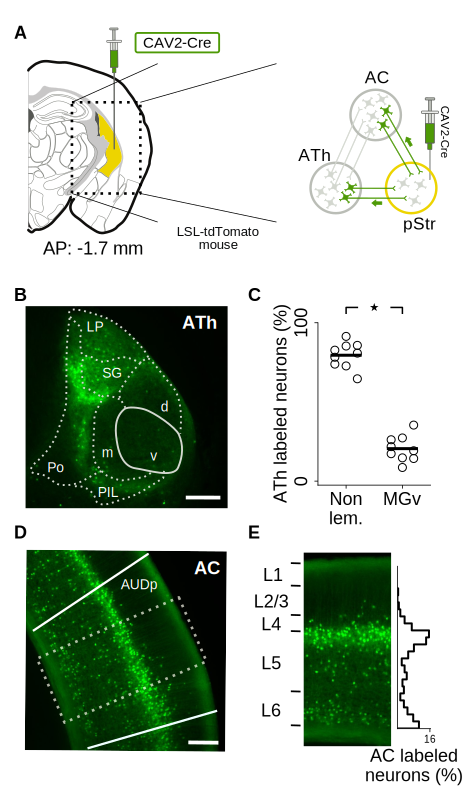
\includegraphics[height=4.1in]{figures/chapter3/fig1_anatomy}% 
  \end{center}
\caption{Neurons in auditory thalamus (ATh) and auditory cortex (AC) project to the posterior striatum (pStr).}{\textbf{(A)} A retrograde virus (CAV2-Cre) was injected in the posterior striatum (yellow) of LSL-tdTomato mice, shown here in a coronal brain slice.  
%
The virus is picked up by the axon terminals and transported to the cell bodies, causing excision of the loxP-flanked STOP cassette and subsequent expression of tdTomato in neurons that project to the injection location. 
%
\textbf{(B)} Expression of tdTomato in ATh neurons (AP -3.16 mm; v, d, and m: ventral, dorsal, and medial nuclei of the medial geniculate body, respectively. LP: lateral posterior nucleus, SG: suprageniculate nucleus, PO: posterior thalamic nucleus, PIL: posterior intralaminar thalamic nucleus).
%
Scale bar = 200 $\mu$m. 
%
\textbf{(C)} Most thalamic striatal-projecting neurons were located in non-lemniscal thalamic nuclei: d, m, SG, LP, PO, and PIL. 
%
Each point represents the fraction of labeled neurons for one of three interleaved sets of histological sections from each animal (3 mice, stars represent p$<$0.05). 
%
\textbf{(D)} Expression of tdTomato in AC neurons (AUDp: primary auditory cortex). 
%
Dotted rectangle represents cortical region shown in E. Scale bar = 200 $\mu$m. 
%
\textbf{(E)} Striatal-projecting neurons in AC were present across deep cortical layers with high density in the superficial portion of layer 5.
%
Results were consistent across all cortical slices analyzed. 
}
\end{figure}
%%%%%%%%%%%%%%%%%%%%%%%%%%%%%%%%%%%%%%%%%%%%%%%%%%%%%%%%%%%%%%%%%%%%%


We next sought to determine how the neurons that project to the striatum respond to sounds. 
%
We used a retrograde viral approach, similar to the technique described above, to tag striatal-projecting neurons with Channelrhodopsin-2 (ChR2).
%
This allowed us to identify these cells during extracellular recording by presenting pulses of blue light \citep{Lima2009} (\fig{\Method}).
%
A key component of this method is separating neurons that are directly activated by ChR2 from neurons that are indirectly activated by feedforward synaptic input. 
%
To achieve this, we applied two previously used criteria: reliability of responses to a train of pulses, and latency of responses to light \citep{Lima2009, Cohen2012}. 
%
To validate this approach, we blocked synaptic transmission locally in a subset of recordings by applying the AMPA glutamate receptor antagonist NBQX (\fig{\MethodDiagram}).
%
This manipulation confirmed that cells which do not respond to 5 Hz trains of light pulses (\fig{\MethodIndirectNoFollow}) or which have long latencies (\fig{\MethodLongLatency}) fail to respond to laser after NBQX, indicating that they were indirectly activated. 
%
Only neurons that were able to reliably follow a train of laser pulses with short latency had light evoked responses that persisted after synaptic transmission was blocked (\fig{\MethodDirectCellAndNBQXPop}).
%
Neurons which passed these criteria were considered directly activated by light, and therefore identified as striatal-projecting neurons (\fig{\MethodSoundCharPop}).

%%%%%%%%%%%%%%%%%%%%%%%% Figure Method %%%%%%%%%%%%%%%%%%%%%%%%%%%%%
\begin{figure}[hp]
  \begin{center}
    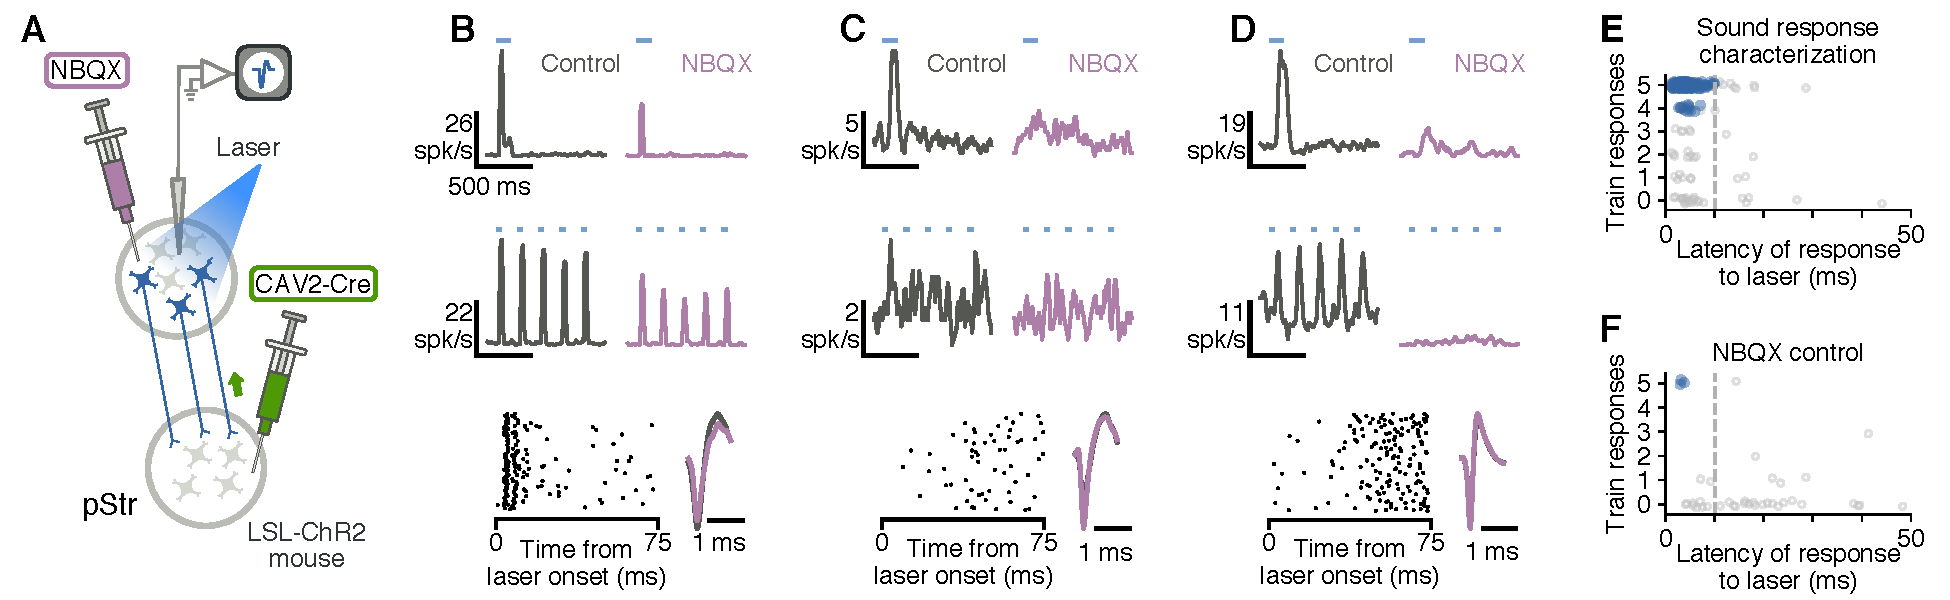
\includegraphics[width=6in]{figures/chapter3/fig2_method}% 
  \end{center}
\caption{Identification of striatal-projecting neurons during extracellular recording.}{\textbf{(A)} CAV2-Cre injected in the posterior striatum (pStr) of LSL-ChR2 mice travels retrogradely and causes expression of ChR2 in striatal-projecting neurons.
%
ChR2-expressing neurons were identified by their responses to laser light during extracellular recording. 
%
To validate approaches for distinguishing between ChR2-expressing neurons and neurons that respond to light due to synaptic excitation, we measured changes in light-evoked responses after blocking synaptic transmission with NBQX.
%
\textbf{(B)} Top row: Response of an example cortical neuron to a 100 ms pulse of blue laser light before and after application of NBQX. Middle row: This neuron responds reliably to a 5 Hz train of 10 ms laser light pulses before and after NBQX. Bottom row: This neuron responds within 10 ms of light onset (left). Spike shape was consistent before and after NBQX injection (right). 
%
\textbf{(C)} Example cortical neuron that responds to light (top) but cannot follow a train of laser pulses (middle). The light-evoked responses of this neuron disappear after NBQX application. 
%
\textbf{(D)} Example cortical neuron that responds to a train of laser pulses (middle) but has a long latency response (bottom). 
%
The light-evoked responses of this neuron disappear after NBQX application. 
%
\textbf{(E)} Neurons collected during sound response characterization recordings were classified as striatal-projecting if they displayed fast, reliable responses to light (blue points). Laser-responsive neurons which did not meet these criteria were excluded (grey points).
Dotted grey line represents a threshold requiring neurons to reach 1/2 of their maximum laser-evoked firing rate within 10 ms.
%
\textbf{(F)} Neurons collected during NBQX control experiments which continued to respond after application of NBQX display fast, reliable responses to light (blue points). Laser-responsive neurons which failed to respond after application of NBQX did not meet the criteria used to operationally define striatal-projecting neurons. 
}
\end{figure}
%%%%%%%%%%%%%%%%%%%%%%%%%%%%%%%%%%%%%%%%%%%%%%%%%%%%%%%%%%%%%%%%%%%%%


To probe the auditory responses of identified striatal-projecting neurons, we used an ensemble of stimuli including bursts of white noise, pure tones at frequencies between 2-40 kHz, and sinusoidally amplitude modulated (AM) white noise at modulation rates between 4-128 Hz. 
%
We recorded the responses of 55 tagged, sound-responsive neurons in auditory thalamus (5 mice) and 45 tagged, sound responsive neurons in auditory cortex (3 mice). 
%
As expected from the anatomical results, a large majority of neurons in auditory thalamus were recorded from non-lemniscal thalamic nuclei (85\%, 47/55, \fig{\NoiseLaserThalLocations}).
%
\fig{\NoiseLaserThalExample} shows an example thalamostriatal neuron which responds reliably to a burst of white noise.
%
\fig{\NoiseLaserACExample} shows the responses to white noise of an example auditory corticostriatal neuron.
%
Although corticostriatal neurons are present in multiple fields of the auditory cortex (\fig{\AnatomyACExample}), our experiments targeted the primary auditory cortex, such that 84\% (38/45) of recorded neurons were from the primary field (\fig{\NoiseLaserACLocations}).

These results demonstrate that both thalamus and cortex send auditory information to the striatum. We next wanted to know whether these two pathways provide redundant or complementary information about sounds to striatal neurons.

%%%%%%%%%%%%%%%%%%%%%%%% Figure Noise/Laser %%%%%%%%%%%%%%%%%%%%%%%%%%%%%
\begin{figure}[hp]
  \begin{center}
    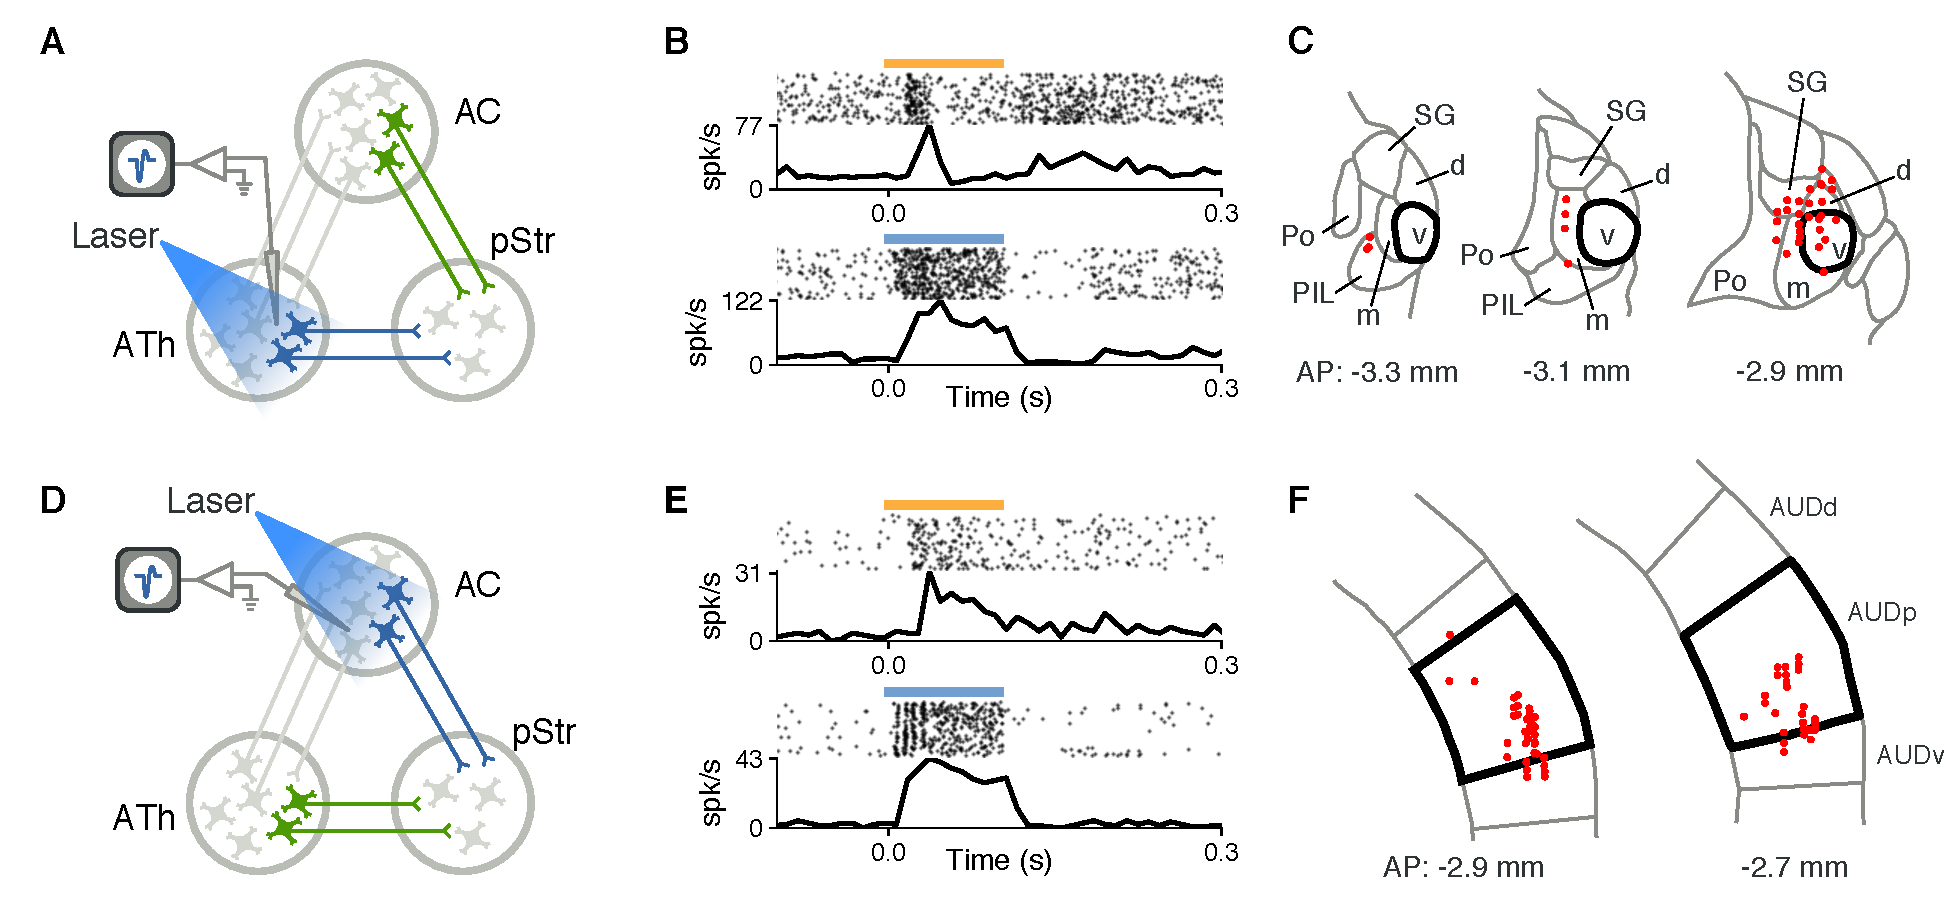
\includegraphics[width=6in]{figures/chapter3/fig3_noise_laser}% 
  \end{center}
\caption{Striatal-projecting neurons in auditory thalamus and auditory cortex display reliable sound responses. 
}{We recorded from ChR2-tagged striatal-projecting neurons in auditory thalamus \textbf{(A)} or auditory cortex \textbf{(D)}.
%
\textbf{(B)} Example sound-evoked response and laser-evoked response from a ChR2-tagged neuron in auditory thalamus (yellow bar: 100 ms burst of 60 dB SPL white noise; blue bar: 100 ms pulse of 445 nm laser light). 
%
\textbf{(C)} Coronal sections showing locations of recorded tagged neurons in ATh. Each recording location was projected onto the closest example section. Thicker lines represent the border of MGv.
%
\textbf{(E)} Same as \textbf{(B)} for an example ChR2-tagged neuron in auditory cortex. 
%
\textbf{(F)} Coronal sections showing locations of recorded tagged neurons in auditory cortex. Each recording location was projected onto the closest example section. Thicker lines represent the border of the primary auditory field (AUDp). AUDd and AUDv are the dorsal and ventral fields, respectively. 
}
\end{figure}
%%%%%%%%%%%%%%%%%%%%%%%%%%%%%%%%%%%%%%%%%%%%%%%%%%%%%%%%%%%%%%%%%%%%%

\subsection{Thalamostriatal and corticostriatal neurons display similar sound frequency tuning bandwidth}

To determine whether thalamostriatal and corticostriatal neurons provide different information about sound frequency to the striatum, we recorded responses of identified neurons from these pathways to pure tones at frequencies between 2-40 kHz and intensities between 15-70 dB SPL. 
%
Figure 3 shows example frequency-intensity tuning curves for a ChR2-tagged neuron in auditory thalamus (\fig{\FrequencyThalExample}) and auditory cortex (\fig{\FrequencyACExample}).
%
We first analyzed the latency of the response to sound, and found that corticostriatal neurons had longer latencies than thalamostriatal neurons (p$<$0.001, Mann-Whitney U test, \fig{\FrequencyLatency}). 
%
Thalamostriatal neurons had higher baseline firing rates than corticostriatal neurons (ATh:Str median=3.75 spk/s, AC:Str median=0.82 spk/sec, p$<$0.001, Mann-Whitney U test). 
%
However, the maximum baseline-subtracted evoked firing rate was not different between thalamostriatal and corticostriatal neurons (ATh:Str median=16.32 spk/s, AC:Str median=11.81 spk/sec, p=0.18, Mann-Whitney U test). 

%%%%%%%%%%%%%%%%%%%%%%%% Figure Frequency %%%%%%%%%%%%%%%%%%%%%%%%%%%%%
\begin{figure}[hp]
  \begin{center}
    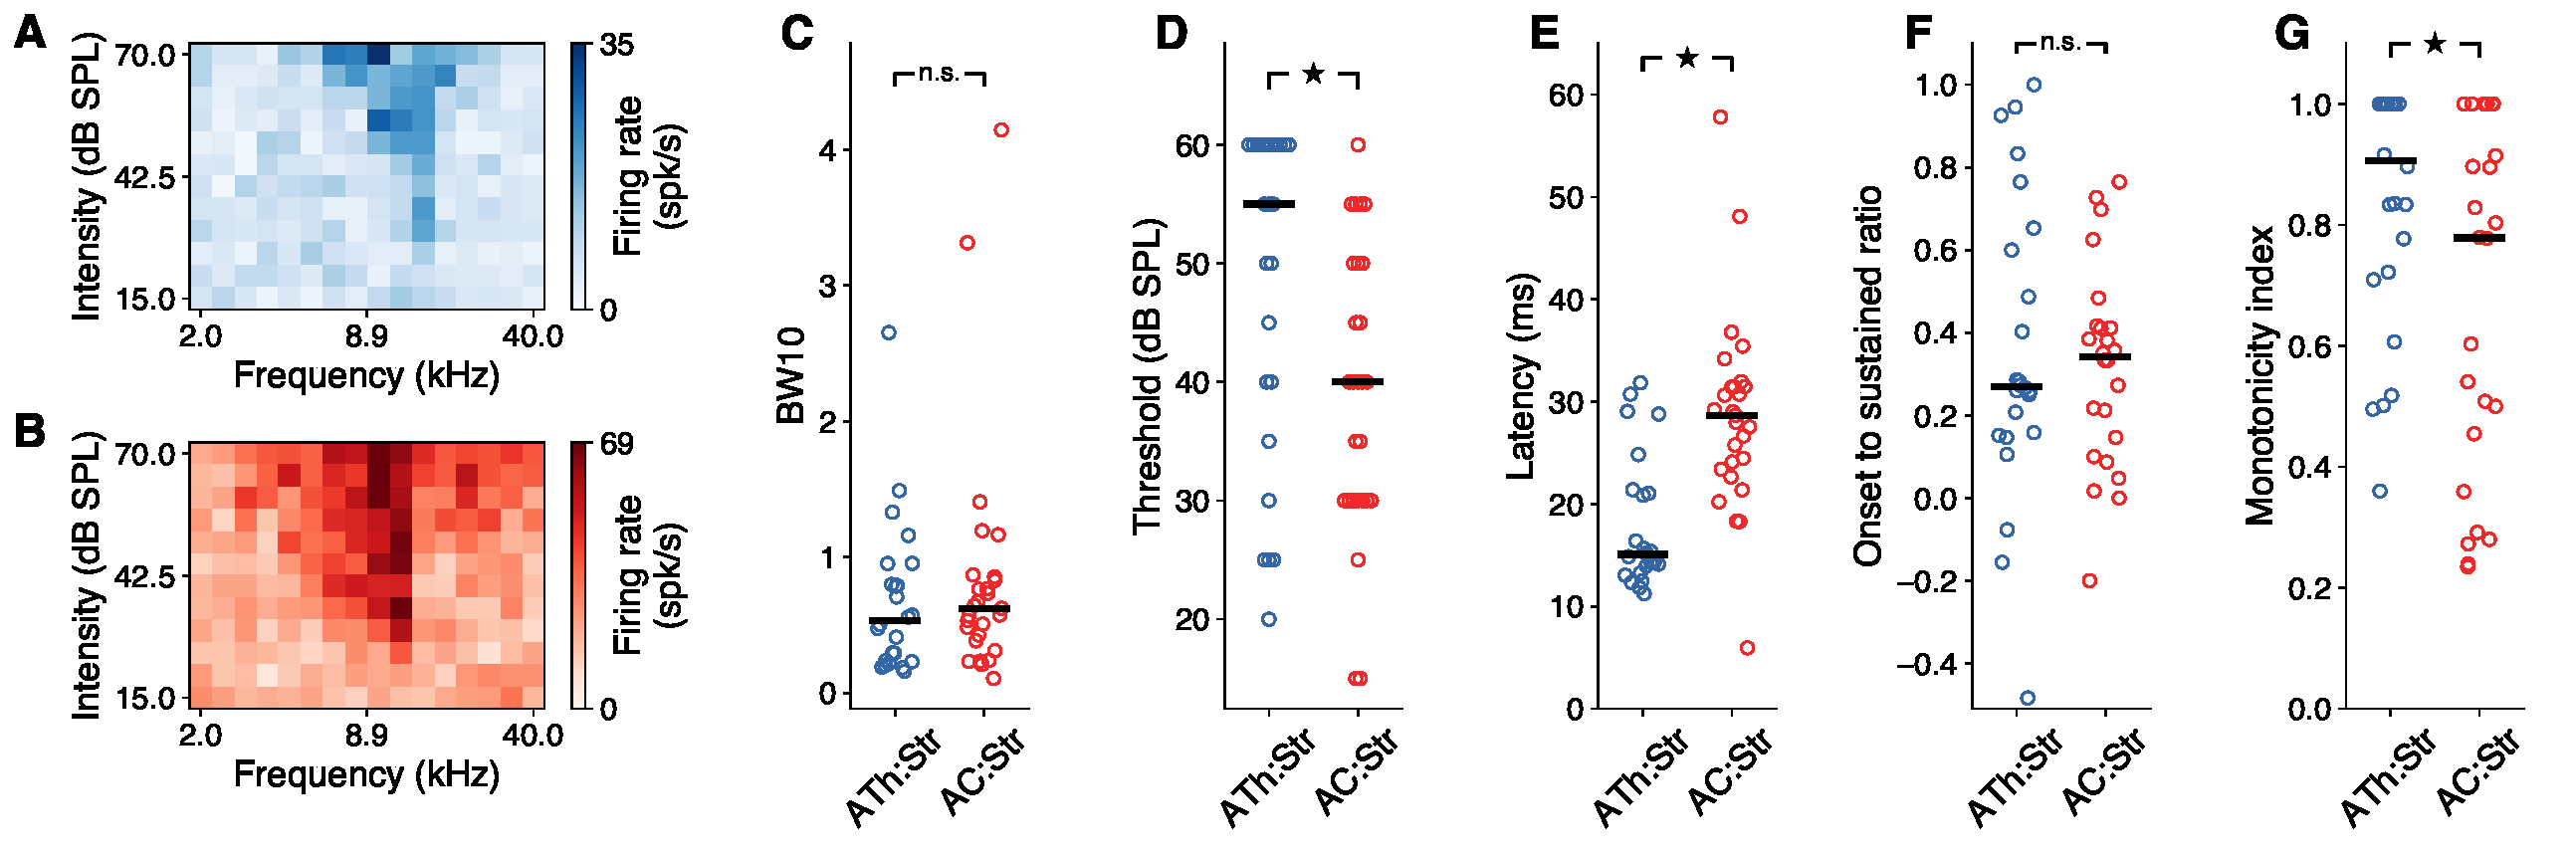
\includegraphics[width=6in]{figures/chapter3/fig4_frequency}% 
  \end{center}
\caption{Auditory thalamostriatal and corticostriatal neurons encode sound frequency with similar fidelity.}{\textbf{(A)} Example frequency-intensity tuning curve from a striatal-projecting neuron in auditory thalamus.
%
Tuning curves were generated by recording neural responses to 100 ms pure tone pips at 16 frequencies (2-40 kHz) and 12 intensities (15-70 dB SPL in 5 dB steps). 
%
\textbf{(B)} Example frequency-intensity tuning curve from a striatal-projecting neuron in auditory cortex. 
%
(C) No statistically significant difference in tuning bandwidth at 10 dB above threshold (BW10) was observed between tuned auditory thalamostriatal (n=24) and auditory corticostriatal (n=27) neurons. 
%
\textbf{(D)} Intensity threshold for responses to pure tones was lower in auditory corticostriatal neurons than thalamostriatal neurons. 
%
\textbf{(E)} Auditory thalamostriatal neurons display shorter response latencies to pure tones than corticostriatal neurons. 
%
\textbf{(F)} No statistically significant difference was observed in the ratio of onset spike rate to sustained spike rate between thalamostriatal and corticostriatal neurons.
%
\textbf{(G)} Thalamostriatal neurons display more monotonic responses to sound level than corticostriatal neurons.
%
Stars represent p$<$0.05. Black bars indicate the median value of each group.
}
\end{figure}
%%%%%%%%%%%%%%%%%%%%%%%%%%%%%%%%%%%%%%%%%%%%%%%%%%%%%%%%%%%%%%%%%%%%%

We then determined the characteristic frequency for each neuron, the threshold sound intensity required to get a response at that frequency, and the bandwidth of the tuning curve at 10 dB above that threshold (BW10). 
%
We found that corticostriatal neurons displayed lower thresholds than thalamostriatal neurons (p=0.015, Mann-Whitney U test, \fig{\FrequencyThreshold})
%
This difference could be the result of convergence from multiple lemniscal and non-lemniscal thalamic inputs onto the cortex. 
%
Calculation of BW10 was only possible for neurons that were tuned for frequency and had thresholds below 60 dB. We found 24 thalamostriatal neurons and 27 corticostriatal neurons that met these criteria.
%
Thalamostriatal and corticostriatal neurons displayed similar BW10 values (p=0.448, Mann-Whitney U test, \fig{\FrequencyBW}) suggesting that the two pathways are capable of providing frequency information to the striatum with similar fidelity. 

Additionally, we estimated how monotonic each neuron was in its response to presentations of the characteristic frequency at different intensities.
%
We found that thalamostriatal neurons displayed responses that were more monotonic with respect to sound level than corticostriatal neurons (p=0.019, Mann-Whitney U test, \fig{\FrequencyMonotonicity}). 
%
Lastly, we evaluated whether temporal response dynamics differed between thalamostriatal and corticostriatal neurons. 
%
We calculated an index that compared the strength of the onset response to sound (the first 50 ms of a neuron's response) with the sustained component of the response (from 50 ms to 100 ms after the beginning of the response). 
%
We found no difference in this index between thalamostriatal and corticostriatal neurons (p=0.845, Mann-Whitney U test, \fig{\FrequencyOnsetivity}). 


Because our method for retrograde ChR2-tagging is not guaranteed to label every striatal-projecting neuron, a subset of untagged neurons may still project to the striatum. Despite this caveat, we evaluated whether there were any differences between tagged neurons and neighboring untagged neurons. We observed no differences in frequency tuning metrics between these populations in either thalamus (BW10: p=0.54, threshold: p=0.28, latency: p=0.39) or cortex (BW10: p=0.79, threshold: p=0.95, latency: p=0.17).

Overall, while thalamostriatal and corticostriatal pathways display different latencies, and corticostriatal neurons are more likely to display non-monotonic tuning for sound level, comparison of BW10 values suggests that both pathways are capable of conveying information about sound frequency to the striatum with similar fidelity. 
%
We next sought to determine how these two pathways encode temporal features of sound.

\subsection{Thalamostriatal and corticostriatal neurons convey different information about temporal features of sounds}

To determine whether thalamus and cortex provide different information about temporal features to the striatum, we analyzed the responses of striatal-projecting neurons to amplitude modulated (AM) noise stimuli at modulation rates from 4 Hz to 128 Hz.
%
We found 36 tagged neurons in auditory thalamus and 24 neurons in auditory cortex with reliable responses to AM noise stimuli.
%
Neurons along the auditory pathway can respond to AM noise by synchronizing their spiking output to the period of the modulation, or by firing during the stimulus presentation without regard to the modulation period.
%
In addition, neurons that synchronize their firing to low AM rates may not do so for high AM rates.
%
Figure 4 shows example responses to AM sounds in two striatal-projecting neurons in auditory thalamus (\fig{\AMThalExamples}) and auditory cortex (\fig{\AMACExamples}).
%
Thalamostriatal neurons synchronized to many of the AM rates presented, but their average firing rate over the duration of the stimulus often depended little on the AM rate.
%
In contrast, corticostriatal neurons appeared less synchronized to the period of the AM stimulus, especially at fast AM rates, and their evoked average firing rate often varied as a function of the AM rate.
%
We found that the ratio of onset to sustained firing rates in response to AM sounds was similar between thalamostriatal and corticostriatal neurons (p=0.23, Mann-Whitney U test).

%%%%%%%%%%%%%%%%%%%%%%%% Figure AM %%%%%%%%%%%%%%%%%%%%%%%%%%%%%
\begin{figure}[hp]
  \begin{center}
    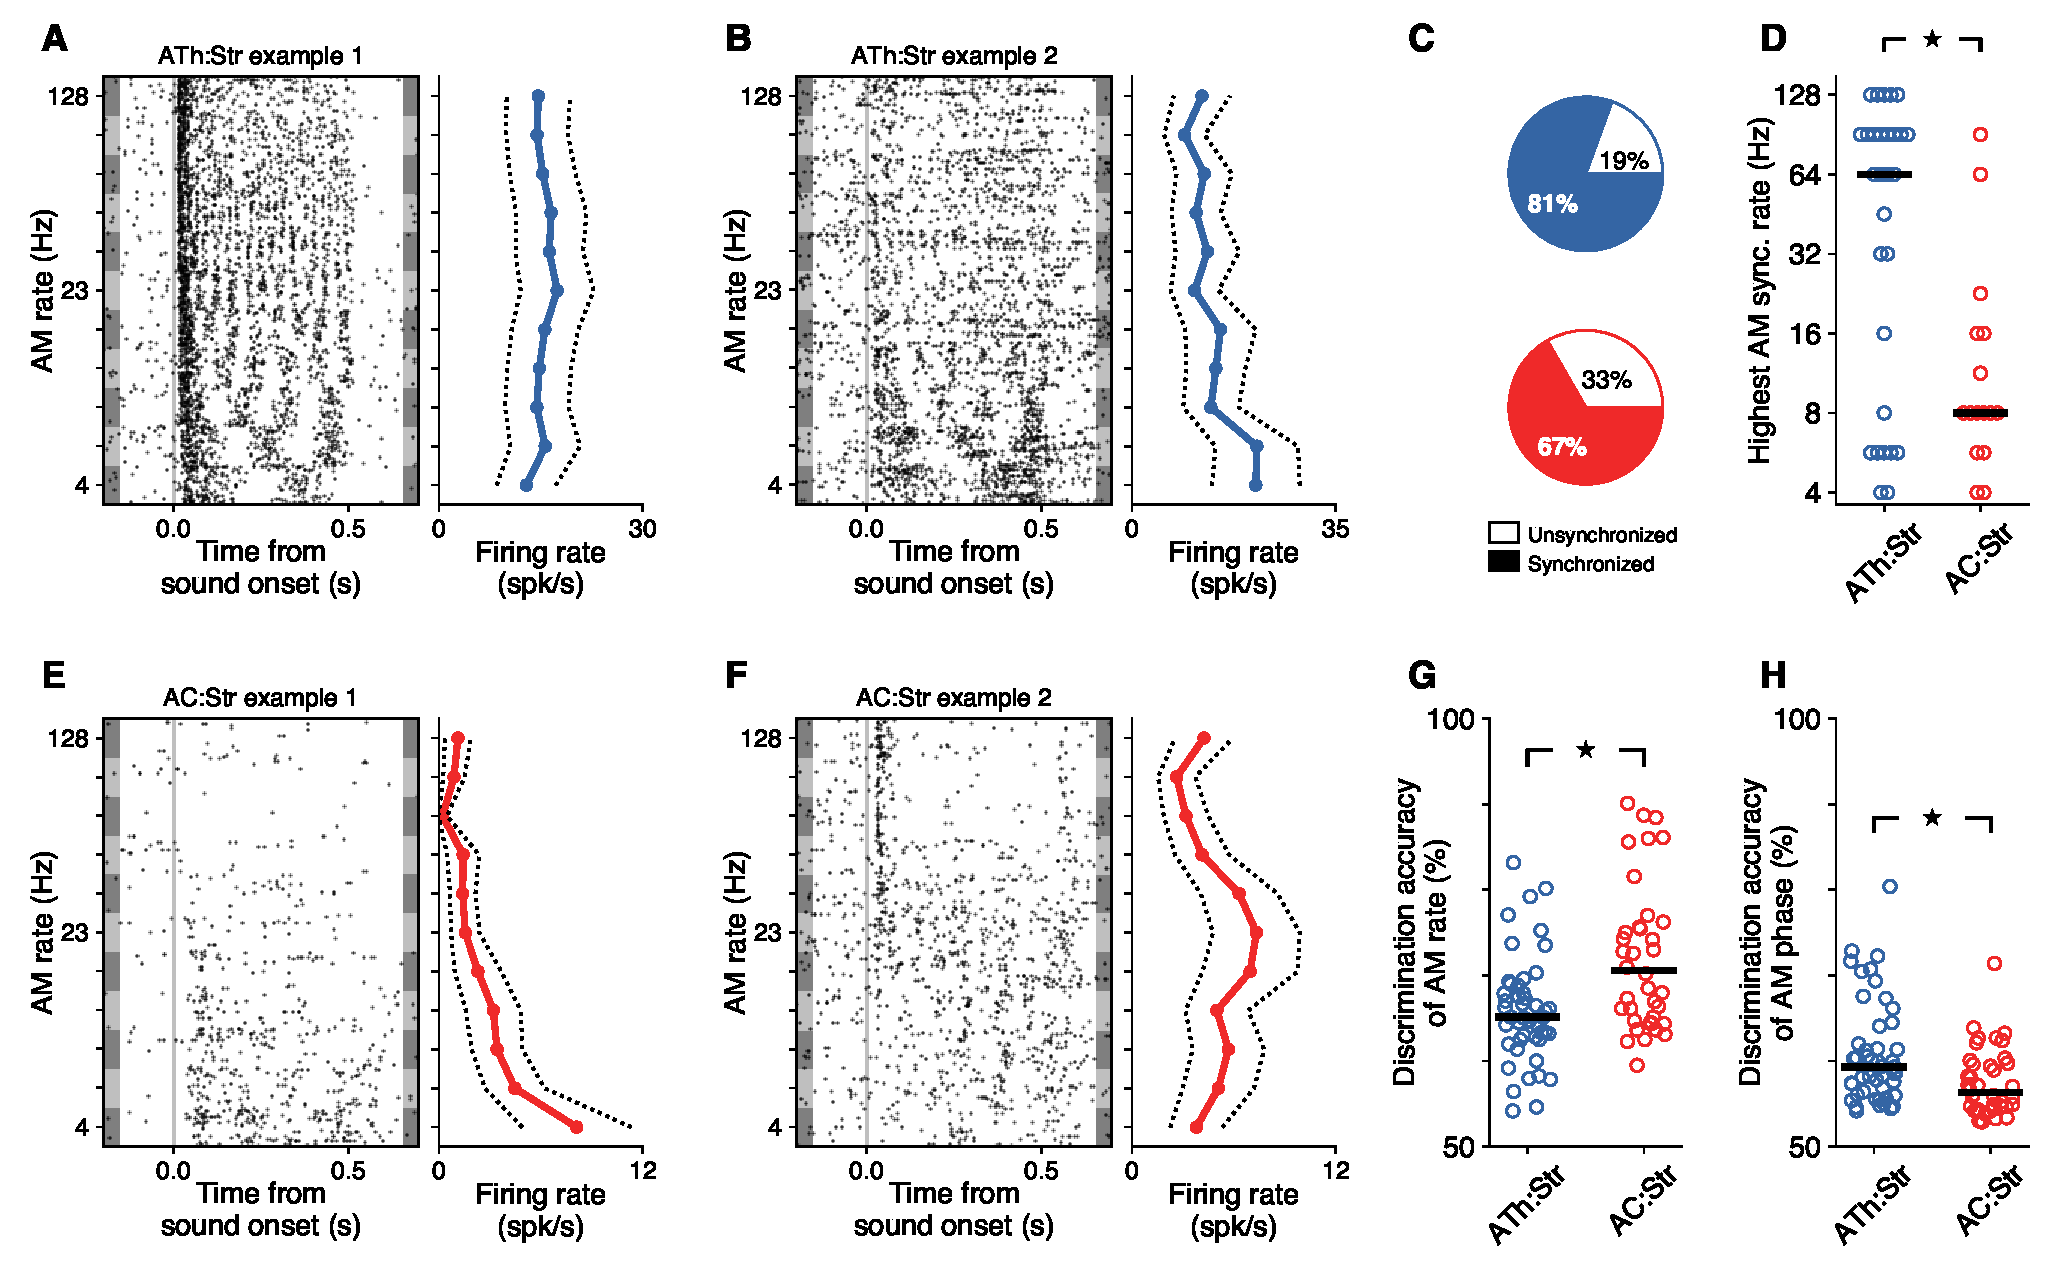
\includegraphics[width=6in]{figures/chapter3/fig5_am}% 
  \end{center}
\caption{Thalamostriatal and corticostriatal neurons convey different information about temporal features of sounds.}{(A, B) Example responses of two auditory thalamostriatal neurons to amplitude modulated (AM) white noise at different modulation rates. 
%
Average firing rates vary little as a function of AM rate. 
%
Dotted lines indicate 1 s.d.
%
AM stimuli consisted of 500 ms bursts of white noise at 60 dB SPL, modulated by a sinusoid (4-128 Hz).
%
Modulation depth was 100\%. 
%
(C) Both thalamostriatal (7/36=19\%) and corticostriatal (8/24=33\%) populations contained some neurons unable to synchronize to any AM stimulus presented. 
%
Filled areas represent neurons able to synchronize to at least one AM stimulus.
%
(D) Thalamostriatal neurons display higher maximum synchronization rates compared to corticostriatal neurons.
%
(E, F) Example responses of two auditory corticostriatal neurons to AM noise at different modulation rates. 
%
Average firing rates are modulated by AM rate. 
%
Dotted lines indicate 1 s.d.
%
(G) A linear discriminator is better able to tell apart preferred from least-preferred AM rate using average stimulus-evoked firing rates of corticostriatal neurons than thalamostriatal neurons. 
%
(H) A linear discriminator is better able to tell apart preferred from least-preferred AM phase using firing rates from thalamostriatal neurons than from corticostriatal neurons. Discrimination accuracy was calculated separately for each AM rate. Each dot represents the average accuracy across all AM rates for each neuron.
%
Stars indicate p$<$0.05. Black bars indicate the median value of each group. 
}
\end{figure}
%%%%%%%%%%%%%%%%%%%%%%%%%%%%%%%%%%%%%%%%%%%%%%%%%%%%%%%%%%%%%%%%%%%%%

To quantify the difference in encoding of AM stimuli between thalamostriatal and corticostriatal neurons, we first determined the highest AM rate to which each neuron was able to synchronize its firing.
%
We found that thalamostriatal neurons were able to synchronize their firing to higher AM rates than corticostriatal neurons (p$<$0.001, Mann-Whitney U test, \fig{\AMSync}).
%
There was also a non-significant trend towards cortical neurons being more likely to show unsynchronized responses to all AM rates we tested: 33\% (8/24) of auditory cortical neurons \emph{vs.}\ 19\% (7/36) of thalamic neurons (p=0.24, Fisher’s exact test, \fig{\AMPies}).
%
These results suggest that auditory thalamostriatal and corticostriatal neurons represent AM sounds in different ways.

To further address these differences in neural representations, we estimated how accurately a downstream linear classifier could discriminate between each neuron's preferred and least-\\preferred AM rate, given average firing rates for each trial.
%
We found that discrimination accuracy was better for corticostriatal neurons than for thalamostriatal neurons (ATh:Str mean=65.9\%, AC:Str mean=72\%, p=0.001, Mann-Whitney U test, \fig{\AMRateDiscrim}).
%
We also calculated discrimination accuracy using spikes only from the sustained portion of the response, and found that this did not affect accuracy in either thalamostriatal or corticostriatal neurons (ATh:Str mean=66\%, ATh:Str with- \emph{vs.} without-onset p=0.68, Mann-Whitney U test. AC:Str mean=70.9\%, AC:Str with- \emph{vs.} without-onset p=0.57, Mann-Whitney U test.)

In addition, to evaluate the amount of information that neurons provide about the full range of AM rates beyond the preferred and least-preferred stimuli, we calculated the mutual information between the response on each trial and the AM rate.
%
We found that corticostriatal neurons provided more information about AM rate than thalamostriatal neurons  (p=0.012, Mann-Whitney U test).
%
Corticostriatal neurons on average provided 0.06 bits of information per trial, with some cells providing up to 0.23 bits. 
%
Thalamostriatal neurons provided an average of 0.03 bits and a maximum of 0.16 bits.
%

We next tested how well a downstream classifier could discriminate between preferred and least-preferred phase of the stimulus envelope.
%
To do this, we aligned each neuron's spikes to the phase of the AM stimulus presented on each trial, and calculated the firing rate during each phase quadrant. 
%
We found that discrimination accuracy for phase was better for thalamostriatal neurons than for corticostriatal neurons (p$<$0.001, \fig{\AMPhaseDiscrim}).
%
We did not observe any differences in AM response metrics between tagged and untagged neurons either in thalamus (highest sync rate: p=0.57, rate discrimination accuracy: p=0.31, phase discrimination accuracy: p=0.75) or cortex (highest sync rate: p=0.27, rate discrimination accuracy: p=0.26, phase discrimination accuracy: p=0.11).

These results suggest that thalamus and cortex provide complementary information about amplitude modulated sounds to the striatum.
%
The average firing rates of neurons in the corticostriatal pathway provide an explicit representation of the modulation rate of a stimulus, while thalamostriatal neurons provide information about the precise timing of acoustic events. 

% DONE: Be consistent about Discussion / Conclusion across chapters
\section{Discussion}

By recording sound-evoked responses of striatal-projecting neurons from auditory thalamus and auditory cortex of awake mice, we found that these two pathways send complementary information about the features of sounds.
%
While thalamic and cortical neurons send largely redundant information to the striatum about sound frequency, thalamostriatal neurons provide signals with shorter latency. 
%
Corticostriatal neurons, meanwhile, are more sensitive to pure tones at low intensities and are more likely to display non-monotonic responses to sound level (\emph{i.e.}, intensity tuning).

Moreover, corticostriatal neurons more accurately represent the amplitude modulation rate in their average firing rate, while the responses of thalamostriatal neurons more closely follow rapid variations in stimulus amplitude.
%
Our results suggest that these two pathways could be differentially recruited during sound-driven behaviors depending on the requirements of the task.

\subsection{Auditory cortical projections to the striatum}
Our anatomical results suggest that neuronal projections from auditory cortex to the posterior striatum in the mouse arise mostly from cortical layer 5, with some projections from layer 6. 
%
These results are consistent with a recent anatomical study in the rat using CAV2 as a retrograde tracer \citep{Jiang2018}, although the projection to striatum from layer 6 was not observed in an earlier study in the rat using a different intersectional viral approach \citep{Znamenskiy2013}. 
%
One challenge with retrograde tracing methods is the possibility of the virus being picked up by damaged fibers of passage. However, it is unlikely that this possibility explains the robust expression seen in cortical layer 6 since our experiments show little expression in MGv, a nucleus which sends neuronal projections to primary auditory cortex that also course through the posterior striatum.

Multiple cortical regions, in addition to the auditory cortex, target the posterior portion of the dorsal striatum \citep{Hunnicutt2016}.
%
Consistent with these anatomical patterns, we observed labeled neurons in cortical regions outside of auditory cortex, including regions of somatosensory cortex overlying the injection site in the posterior striatum.
%
The presence of labeled neurons outside the desired auditory cortical region raises the possibility that the virus spread beyond the target striatal area (\emph{e.g.}, by leakage along the injection tract). However, because expression was restricted to the same laminar distribution observed in auditory cortex, the possibility of major leakage does not seem likely, as this would result in less organized patterns of expression of the fluorophore.

\subsection{Representation of sound features across the auditory pathway}
%
Previous studies in anesthetized animals comparing neurons in auditory cortex and lemniscal auditory thalamus have found little difference in frequency tuning bandwidth between these regions \citep{Miller2002}. 
%
Within the thalamus, frequency tuning bandwidth differs between the dorsal (MGd) and ventral (MGv) nuclei of the medial geniculate body, while other nuclei (MGm and POL) show overlapping tuning with MGv \citep{Anderson2011}.
%
Consistent with previous studies \citep{Doron1999}, our anatomical results indicate that the thalamostriatal projection largely originates from neurons across non-lemniscal nuclei. 
%
These observations imply that, without the ability to record directly from striatal-projecting neurons, it would be challenging to predict what frequency information is conveyed by these neurons. 
%

Our results indicate that, although some thalamostriatal neurons are located in MGd, frequency tuning bandwidth between thalamostriatal and corticostriatal neurons is largely overlapping. 
%
Despite the similarity in tuning bandwidth we observe between thalamostriatal and corticostriatal neurons, it is possible that the relative effects of cortical and thalamic pathways on striatal responses are additionally shaped by the strength of the synapses in these pathways and by the patterns of convergence onto striatal neurons to produce appropriate behavioral outputs. 
%
For instance, differences in release probability and short term plasticity have been shown between thalamostriatal and corticostriatal synapses \citep{Ding2008}, and these two pathways target different compartments of striatal cells \citep{Smith2004}. 
%
Notably, with the parameters used in this study, we were not able to calculate BW10 for many thalamostriatal neurons (56\%, compared to 40\% of AC:Str neurons) because either CF was not captured, or we had no data for 10 dB above threshold. This suggests that tuning may be more common among corticostriatal neurons across the range of intensities tested.
 
The responses to amplitude modulated (AM) sounds that we observed across cortex and thalamus are consistent with previous work showing that responses to these sounds change from being synchronized with the stimulus at the auditory periphery to being largely unsynchronized in higher auditory cortical areas (reviewed in \cite{Joris2004} and \cite{Wang2008}). 
%
For example, in primates, neurons in A1 have mixed temporal (synchronized) and rate-coded (unsynchronized) representations, while responses of most neurons in secondary auditory fields do not synchronize to the period of the modulation \citep{Bendor2007, Niwa2013}.

In the auditory thalamus, the representation of AM stimuli differs across nuclei. 
%
MGm and SG display largely synchronized responses, MGd displays responses that are largely unsynchronized, and MGv displays a mixture of the two response types \citep{Bartlett2013}. 
%
Given these results, the thalamostriatal pathway could contain a mixture of different AM response types. 
%
Our experiments, using a method to interrogate neurons specifically from this pathway, suggest that synchronized responses predominate among thalamic neurons that project to the striatum.

In neural circuits responsible for discriminating AM rate, having inputs where the overall spike count is highly correlated with AM rate (as seen in corticostriatal neurons) means a simple threshold can accomplish the discrimination task. 
%
In contrast, inputs in which firing is synchronized with the variations in amplitude, but that do not change the overall spike-count for the duration of the stimulus (as is common in thalamostriatal neurons), would require additional processing for implementing AM rate discrimination.
%
As representations of AM sounds are transformed from synchronized to rate-coded across the auditory pathway, these signals become progressively more useful to an area performing AM rate discrimination.

\subsection{Subcortical outputs of the auditory thalamus}
%
The posterior striatum is not the only subcortical region where auditory thalamic and cortical signals converge.
%
The lateral amygdala, the most extensively studied subcortical output of the auditory thalamus, also receives extensive inputs from auditory cortex \citep{Ledoux2000}.
%
%
The thalamoamygdala pathway is capable of exhibiting learning-induced changes in synaptic strength thought to underlie amygdala-dependent aversive conditioning \citep{McKernan1997}.
% 
Lesions to the entire auditory thalamus disrupt fear conditioning to sounds, but lesions to either the corticoamygdala or the thalamoamygdala pathway alone leave fear conditioning intact \citep{Ledoux1983, Romanski1992}.
% 
Thus, the thalamoamygdala and the corticoamygdala pathways are both independently able to facilitate fear conditioning. 
%
Similarly, auditory discrimination tasks involving simple, narrowband stimuli require posterior striatal circuits \citep{Guo2018} but can be performed after extensive lesions of auditory cortex \citep{Gimenez2015}, suggesting that auditory corticostriatal and thalamostriatal pathways are independently able to mediate this discrimination. 

Our results suggest that thalamic neurons that project to the striatum are located in many of the same nuclei as neurons that project to the lateral amygdala \citep{Doron1999}. 
%
Although neurons in the amygdala encode both negative and positive valence of sensory cues \citep{Tye2008}, these neurons seem to play only a minimal role in associations between stimuli and actions to obtain reward \citep{Baxter2002}. 
%
Regions of the dorsal striatum, in contrast, have been shown to play a key role in reward-related motor learning \citep{Wickens2003, Balleine2007}.
% 
These differences suggest that the thalamostriatal and thalamoamygdala pathways play complementary roles in sound-driven behavior. 

%
Thalamic projections to subcortical forebrain structures are predominant in phylogenetically primitive vertebrates with less developed neocortices \citep{Ebner1969, Kudo1986}, and it is likely that the last common ancestor between mammals and other vertebrates displayed similar neural pathways. 
%
This suggests the possibility that the outputs from the auditory thalamus to the striatum and amygdala in mammals are vestigial, an evolutionary holdover. 
%
However, we find that the thalamostriatal and corticostriatal pathways send complementary information about sound features to the striatum. 
%
Therefore, by using information arriving from the thalamus, rather than signals from cortex alone, striatal circuits might help achieve better performance in certain kinds of auditory tasks.

\subsection{Striatum-mediated learning with sensory inputs from two parallel pathways}

Recent studies have proposed a model of reward-related sound discrimination learning in which the synapses between auditory cortical neurons that represent a stimulus feature and neurons in the striatum that can drive appropriate actions are potentiated \citep{Xiong2015}. 
%
While it is not known whether thalamostriatal synapses undergo the same type of stimulus-specific plasticity, thalamic signals (potentially via the striatum) seem sufficient to mediate associations between narrowband sounds and rewarded actions \citep{Gimenez2015, Guo2018}.
%

Depending on the demands of a task, striatal neurons may selectively potentiate distinct input sensory pathways.
%
For tasks requiring discrimination between AM rates, the cortical inputs provide signals that can be decoded with a linear classifier without further processing.
%
In contrast, for tasks requiring precise timing, striatal neurons could potentiate thalamic inputs and take advantage of the features provided by this pathway. 

\section{Link to Chapter IV}
In this chapter, we compared the auditory information sent to the posterior striatum by the parallel corticostriatal and thalamostriatal pathways.
%
We found that the two pathways provide frequency information to the posterior striatum with similar fidelity, but that they differ in their representation of temporal modulations in sound amplitude. 
%
While neurons in the thalamostriatal pathway more often represented AM rate by synchronizing their firing rate to the stimulus envelope, neurons in the corticostriatal pathway were more likely to fire in an unsynchronized manner, but to fire more spikes over the duration of the stimulus for particular AM rates. 
%
We hypothesized that this rate-coded representation of AM rate is more useful to downstream circuits performing AM rate discrimination, because it enables discrimination to be performed by a simple linear decoder. 
%
To test this hypothesis, we designed a behavioral task to evaluate whether chemical inactivation of auditory cortex has a greater effect on AM rate discrimination than on frequency discrimination. 
 % Pathway recording
% LATER: I need a figure with some psychometric showing good performance. 
% Some cool additional analysis that would be nice to include if I have time. 
%LATER: How long does it take to learn the categorization once the initial exemplars are learned? 
%LATER: How long does it take to learn to switch after you are able to categorize? 
%LATER: How long does it take to learn the second category after you are able to learn the first? 

% Figures in this chapter
\newcommand{\Task}{1}
\newcommand{\TaskDiagram}{\Task A}
\newcommand{\TaskTrials}{\Task B}
\newcommand{\TaskSounds}{\Task C}

\newcommand{\Training}{2} 
\newcommand{\TrainingSessions}{\Training A}
\newcommand{\TrainingTrials}{\Training B}

\newcommand{\AmodEffect}{3}
\newcommand{\amodPsychometrics}{\AmodEffect A, B, D, E}
\newcommand{\amodCorrect}{\AmodEffect C, F}

\newcommand{\SingleSound}{4}
\newcommand{\SinglePsy}{\SingleSound A, C}
\newcommand{\SingleSum}{\SingleSound B, D}
\newcommand{\SingleFreqP}{\SingleSound A}
\newcommand{\SingleFreqS}{\SingleSound B}
\newcommand{\SingleAMP}{\SingleSound C}
\newcommand{\SingleAMS}{\SingleSound D}

\chapter{A behavioral task for evaluating the cortical and subcortical
contributions to sound feature discrimination}

\section{Introduction}
% We found that corticostriatal and thalamostriatal pathways send different
% information about certain sound features to the striatum. 
% DONE: Chapter number
In \ch{\Thstr}, we found that the thalamostriatal and corticostriatal
pathways send complementary information to the striatum about some features of
sound. 
%
While both pathways conveyed frequency information to the striatum with similar
fidelity, corticostriatal neurons better represented the rate of temporal
amplitude modulations in their overall spiking rate.
%
The spiking rate of thalamostriatal neurons more closely followed rapid
variations in stimulus amplitude, but the total number of spikes during the
stimulus was less indicative of the modulation rate.
% What is the significance of this difference? 
% DONE: Chapter number
While our earlier experiments in \ch{\Musc} strongly suggested a role for the
striatal target region of these projections in sound-guided behavior, the
relative contribution of these parallel pathways to behavior is unclear. 
%

% Some inactivation studies show that AM discrimination suffers after cortical
% lesions.
Lesion studies have suggested that discrimination of fast AM rates suffers
following removal of auditory cortex \citep{Deutscher2006}.
%
In contrast, sound frequency discrimination behavior has been shown to persist
after extensive lesions of AC \citep{Gimenez2015}.
%
% DONE: Phrase as either/or cortical/subcortical?
We therefore hypothesized that the cortical representation of AM is necessary
for accurate AM discrimination, but that sound frequency discrimination can be
accomplished with auditory information from the subcortex alone. 

% Specific hypothesis and test
Specifically, we hypothesized that the effect of reversible AC inactivation
would be greater on AM discrimination than on frequency discrimination. 
%
To test this hypothesis, we designed and implemented a behavioral task that
permits evaluation of the effects of a single reversible inactivation on
discriminations of both sound features.
%
We performed bilateral reversible inactivations of AC in animals trained on
this task, and found that discrimination of both features was impaired. 
%
While the contribution of the thalamostriatal and corticostriatal pathways to
discrimination of these sound features is still not clear, this task provides a
method for comparing the effect of reversible chemical manipulations on
discriminations of diverse stimulus features. 


\section{Methods}

\subsection{Animal subjects}
% DONE: Number of mice
14 adult male wild-type mice (C57/BL6J) were used in this study. Mice had ad
libitum access to food, but water was restricted. Free water was provided on
days with no experimental sessions. All procedures were carried out in
accordance with National Institutes of Health standards and were approved by
the University of Oregon Institutional Animal Care and Use Committee.

\subsection{Behavioral task}
% DONE: Update methods for amod task
Behavioral data was collected using the taskontrol platform
(\url{www.github.com/sjara/taskontrol}) developed in our laboratory using the
Python programming language (\url{www.python.org}).
%
Mice initiated each trial by poking their noses into the center port of a
three-port behavior chamber.
%
% DONE: We aren't making animals wait - check the paradigm After a silent delay
% of random duration (150-250 ms, uniformly distributed), a sound was presented
% for 500 ms.
%
The sound was either a narrow-band sound (chord), a single tone, or a
sinusoidally-amplitude-modulated white noise.
%
The decision to use chords or tones was chosen by the experimenter, and
thereafter during the behavior session the type of stimulus alternated between
cords/tones and AM sounds each trial (stimulus type was not randomized per
trial).
%
Animals were required to stay in the center port until the end of the sound and
then chose one of the two side ports for reward (2 $\mu$l of water) according
to a reward contingency that was specific to the type of sound.
%
For chords and tones, the reward contingency was: low frequency: go to left
port; high frequency: go to right port.
%
For amplitude-modulated noise, the reward contingency was: slow modulation
rate: go to left port; fast modulation rate: go to right port.
%
If animals withdrew before the end of the stimulus, the trial was aborted and
ignored in the analysis.
%
Chord stimuli were 12 simultaneous pure tones logarithmically spaced in the
range f/1.2 to 1.2f for a given center frequency f.
%
Within a behavioral session, we used 8 distinct center frequencies for chords
and tones, and 8 distinct modulation rates for AM sounds.
%
Each behavioral session lasted 60 to 90 minutes.

\subsection{Muscimol inactivation}
% DONE: Change to match muscimol protocol for amod study.  @internet
Bilateral craniotomies were performed under stereotactic surgery over the
posterior striatum (1.7 mm posterior to bregma, 3.55 mm lateral from midline)
of mice trained in the two-alternative choice sound discrimination task.
%
Headbars were implanted to allow for head-fixation.
%
Each craniotomy was protected with a plastic ring and filled with silicon elastomer (Sylgard 170, Dow Corning).
%
Animals were allowed to recover for at least 3 days before resuming behavioral training.
%
Following recovery, implanted animals were trained on the sound discrimination task until they reached their pre-surgery performance level before beginning muscimol inactivation.

For intracranial injection, we used glass pipettes (5 $\mu$l Disposable Micropipettes, VWR) pulled and trimmed to an inner diameter of 15-20 micrometers at the tip.
%
Animals were head-fixed and allowed to run on a wheel during the injection.
%
Craniotomies were exposed by removing the silicon elastomer covering, and a glass pipette filled with reagent (either muscimol or saline) was lowered into the brain to a depth of 3.1 mm from brain surface using a micromanipulator.
%
A volume of 45 nl of muscimol (0.25 mg ml$^{-1}$, final dose of 11.25 ng per bolus) was injected under air pressure in each hemisphere at a rate of 90 nl min$^{-1}$, twice per hemisphere.  %
%
One injection was given first at the front of the right craniotomy, then the front of the left craniotomy, then the rear right, and finally the rear of the left craniotomy. 
%
% Given the relationship between concentration and diffusion distance (from
% Fick's law) and previous reports of muscimol effects on neuronal activity
% \citep{Edeline2002}, we expect that by the first 10 minutes of the behavioral
% session, the effects of muscimol (50\% reduction in firing or more) will be
% confined to a volume smaller than 1 mm in diameter centered at the injection
% site. This volume matches well the extent of the posterior tail of the
% striatum (approx. 1 mm A-P, 0.6 mm M-L, 1.5 mm D-V) that receives auditory
% inputs \citep{Hunnicutt2016}.
%
The pipette was left in place for 60 seconds following each injection, then raised 0.5mm and left in place for another 60 seconds before being removed.
%
The entire injection procedure was completed within 30 minutes.
%
The craniotomies were then protected with a new silicon elastomer cap, and the mouse was placed back into its home cage for 30 minutes before starting the behavior session.
%
After collection of 4 saline sessions and 4 muscimol sessions, 45 nl of fluorescent dye (DiI, Thermo Fisher Scientific) was injected at the same injection coordinates.
%
Animals were then perfused transcardially with 5\% paraformaldehyde, and brains were extracted and postfixed for 12-24 hours.
%
Brains were then sliced (100 um) and imaged to verify the location of fluorescent dye injection.  

\subsection{Analysis of behavioral data}

% DONE: Add stuff about the GLMER models here.
Psychometric curve fitting was performed via constrained maximum likelihood to estimate the parameters of a logistic sigmoid function (\url{http://psignifit.
%
sourceforge.net}). Statistical comparisons were performed using non-parametric statistical tests with no assumption of normality. 
%
Generalized linear mixed models were fit with the R programming language (\url{https://www.r-project.org/}) using the `lme4' package (\url{http://lme4.r-forge.r-project.org/}).


\section{Results}

% DONE: Table number
We found that this task was challenging to learn, but that animals could learn to perform it well if given sufficient training time.
%
We used a set of criteria defined in Table IV.1 to determine when mice were ready to advance to the next training step.
%
Animals first advanced through a series of behavioral stages designed to familiarize them with the behavior box and begin to teach them the rules of the task.
%
During the first stage, animals received a water reward after poking their nose
in any of the three ports in the box.
%
This stage allowed animals to learn that the behavior box is a good place to
be, and engaged their natural desire to explore to teach them that they are
able to control the environment and trigger changes by poking in the ports.
%%%%%%%%

%%%%%%%%
In the next stage, animals had to poke in the center port and then go to the
side ports to collect water.
%
This stage began to teach the animals that the center port is where you go to
trigger trials, and that going to a side port is how you collect reward.
%
During these first two stages, an auditory stimulus was played to the animals when they triggered a trial by sticking their nose in the center port.
%
After animals were acquainted with the box and the idea of poking to receive water, they began to learn the sound-action association.
%
% DONE: Mention sound above
During the next stage, animals triggered a trial by poking in the center port,
and then had to go to the right port to collect a reward if the AM rate of the
presented sound was fast, and to the left port if the AM rate was slow.
%
However, on this stage animals were guided towards forming the correct
association by letting them correct their choice if they first made a mistake.
%%%%%%%%

%%%%%%%%
After animals performed well on this stage, we started requiring animals to
make a correct choice on the first try.
%
% DONE: define the range
When they were performing well on this stage, we began presenting a range of AM
rates between the previously-trained fast and slow rates (usually 8 rates,
logarithmically-spaced between the slow and fast rate used in the initial training).
%
During this stage, animals had to learn the category boundary between the
``fast'' and ``slow'' rates.
%
Once they became proficient at this discrimination, animals had good knowledge
of the task structure and rules.
%
At this point, we began to train on two narrow-band stimuli (or pure tones for
some animals).
%
We then switched to a stage where we presented a range of frequencies, logarithmically-
spaced between the initial low and high frequency, and
trained animals until they had learned the boundary between ``high'' and
``low'' sound frequencies as well.
%
% DONE: At this point is ambiguous does it mean this or the next one?
After they had been trained to categorize first AM rate, and then frequency of sound,
we started to introduce the next level of task complexity.
%%%%%%%%

%%%%%%%%
During the next training stage, the type of sound presented when animals
triggered a trial switched between an AM noise and a narrow-band chord (or pure
tone) every other trial.
%
% DONE: Takes little time to do, which is a cool feature. Talk about that here. 
The sound-action association necessary to receive reward was the same as had
been previously learned for each sound.
%
We first introduced animals to the type of sound switching by presenting only
two examples of each sound type, but then moved on to presenting a range of AM
rates and sound frequencies.
%%%%%%%%

%
% LATER: Number of sessions it took to learn the switching.
% Animals took few sessions to learn to switch back and forth between the types 
% of stimuli they were categorizing.
%%%%%%%%%%% Training structure table %%%%%%%%%%%%%%

%DONE: Last criterion to advance (to experiment ready)
After animals performed above 80\% correct on each discrimination for 3 consecutive training sessions, they were deemed ready for use in experiments. 
%
Animals took an average of 119 sessions (\fig{\TrainingSessions}) and performed an average of 100,892 trials (\fig{\TrainingTrials}) before they were deemed ready for experiments.

\begin{sidewaystable}
%\begin{table}
\resizebox{\textwidth}{!}{%
\begin{tabular}{lllll}
\textbf{Stage} & \textbf{Name}        & \textbf{Goal}                           & \textbf{Water delivery}       & \textbf{Criterion to advance}              \\
SD AM          & Sides Direct, AM     & Get animals to poke and collect water   & After center or side poke     & One session with 200 rewards               \\
D AM           & Direct, AM           & Trial initiation in center poke         & After center poke             & One session with 200 rewards               \\
NC AM          & On next correct, AM  & Discover correct association            & After correct/ed side poke    & One session with 500 rewards               \\
IC AM          & If correct, AM       & Enforce correct association             & After correct side poke       & Animal performs \textgreater{}80\% correct \\
P AM           & Psychometric, AM     & Categorize AM rate                      & After correct side poke       & Animal performs \textgreater{}80\% correct \\
IC F           & If correct, Freq     & Form association for frequency          & After correct side poke       & Animal performs \textgreater{}80\% correct \\
P F            & Psychometric, Freq   & Categorize sound frequency              & After correct side poke       & Animal performs \textgreater{}80\% correct \\
IC M           & If correct, Mixed    & Switch between sound types              & After correct side poke       & Animal performs \textgreater{}80\% correct \\
P M            & Psychometric, Mixed  & Categorize both sound types             & After correct side poke       & Three sessions \textgreater{}80\% correct \\
\end{tabular}}
%DONE: Table caption (just review it one more time before nobody ever sees it again). 
\caption{Stages of behavioral shaping.}{Animals progressed through 9 behavioral training stages during behavioral shaping.
%
Each stage was designed to teach the animal a new feature of the behavioral task.
%
Animals graduated to the next phase of training when they performed above a set criterion level.
%
Over the first three training stages, animals primarily learned about the behavioral box and the structure of the task.
%
After an initial session where a nose poke in any of the three ports would trigger water, animals next had to learn to trigger rewards by poking in the center and then collecting the reward at the side.
%
The sound-action association was trained over a series of three stages, where animals could initially correct a previous incorrect response and still get a reward.
%
After this stage, a correct response was required on the first poke.
%
Once animals were capable of performing the discrimination behavior with two prototype stimuli (well-separated in stimulus space), they were then tested with a range of stimuli logarithmically-spaced between the initial two prototypes, and were required to learn the category boundary.
%
Finally, once animals were capable of categorizing both AM rate and sound frequency, the sound triggered by every nose poke began to alternate between an AM noise stimulus and a tone every other trial.
%
Animals still had to perform the previously-learned categorization on each stimulus.}
\end{sidewaystable}
%\end{table}

%%%%%%%%%%%%%%%%%%%%%%%%%%%%%%%%%%%%%%%%%%%%%%%%%%%


% \subsection{Animals can switch between discriminations of different stimulus
% features every trial}
% 
% Despite the difficulty of learning this task, which was evident by the long
% time required for animals to progress through all of the many training stages,
% animals were able to achieve high levels of performance.
% NO: I need a figure with some psychometric showing good performance. 

%%%%%%%%%%%%%%%%%%%%%%%% Figure Task %%%%%%%%%%%%%%%%%%%%%%%%%%%%%
\begin{figure}[hp] \begin{center}
	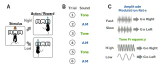
\includegraphics[width=6in]{figures/chapter4/figure_task} \end{center}
	\caption{A behavioral task for evaluating the effects of reversible
	inactivation on discrimination of different sound
	features.}{\textbf{(A)} Schematic of the two-alternative choice sound
	feature discrimination task. Mice initiated each trial by entering a
	center port and had to choose one of two side reward ports depending on
	the sound presented.
	%
\textbf{(B)} The type of sound presented was alternated every other trial. 
%
% DONE: Make sure all other figure captions have bold cap labels
\textbf{(C)} On trials when an AM noise stimulus was presented, mice had to
choose the right reward port if the modulation rate was fast and the left
reward port if the modulation rate was slow to be rewarded. On trials when a
narrow band chord was presented, mice were rewarded for picking the right port
if the sound frequency was high and the left port if the sound frequency was
low. 
%
}
\end{figure}
%%%%%%%%%%%%%%%%%%%%%%%%%%%%%%%%%%%%%%%%%%%%%%%%%%%%%%%%%%%%%%%%%%%%%

% DONE: I think this figure should come earlier. 
%%%%%%%%%%%%%%%%%%%%%%%% Figure Training Time %%%%%%%%%%%%%%%%%%%%%%%%%%%%%
\begin{figure}[hp] \begin{center}
	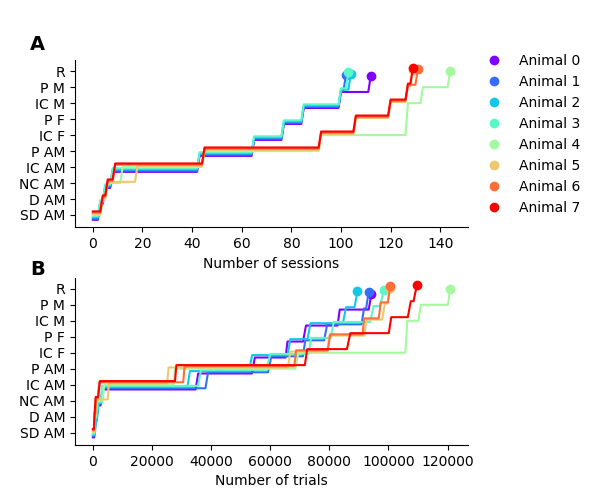
\includegraphics[width=6in]{figures/chapter4/figure_training}%
\end{center} \caption{Animals took about 4 months to learn the
task.}{\textbf{(A)} Animals progressed through 9 training steps over an average
of 119 behavioral training sessions before being ready for experiments (min:
102 sessions; max: 144 sessions). 
%
\textbf{(B)} Animals performed an average of 100,892 trials before being ready
for experiments (min: 89,527; max: 120,885). 
%
} \end{figure}
%%%%%%%%%%%%%%%%%%%%%%%%%%%%%%%%%%%%%%%%%%%%%%%%%%%%%%%%%%%%%%%%%%%%%

\subsection{Reversible inactivation of AC affects discrimination of both sound
frequency and AM rate}

After animals had learned the task, we began performing
bilateral intracranial injections of either the GABA agonist muscimol, or a
saline control, 30 minutes before each behavioral sessions.
%
We alternated between muscimol and saline injections each day. 
%
Muscimol injection affected performance on both tone and AM trials, resulting
in both a flattening of the psychometric curve (\fig{\amodPsychometrics}) and a
reduction in overall performance (\fig{\amodCorrect}) for both animals tested. 
%
We tested the hypothesis that muscimol has a stronger effect on AM
discrimination performance than on frequency discrimination performance by
comparing two generalized linear mixed effect regression models, both attempting
to explain the variance in correct response likelihood that was explained by the
identity of the injection (saline \emph{vs.} muscimol). 
%
In the null model, we allowed the intercept to differ between data from the two
sound types.
%
This inclusion of a random intercept for different sound types helped to account for the fact that animals often performed much better on the
frequency discrimination trials than on AM discrimination trials.
%
Against this null model we compared a model which allowed both random
intercept for sound type, allowing for the fact that performance started
at a different level, as well as allowing for random slopes (a difference in
the strength of the effect between the two sound types).
%
For both models we additionally allowed the slope and intercept of the muscimol
effect to vary between the animals included in the comparison (n=2). 
%
Allowing for random slopes of the effect of muscimol based on sound type did
not significantly increase the variance explained by the model
($\chi^{2}$=1.64, p=0.44).
%
Therefore, we fail to reject the null hypothesis that the strength of the
muscimol effect is the same for discrimination of frequency and AM rate. 

% Inactivation caused deficits in discrimination of both types of stimuli.
\begin{figure}[hp] \begin{center}
    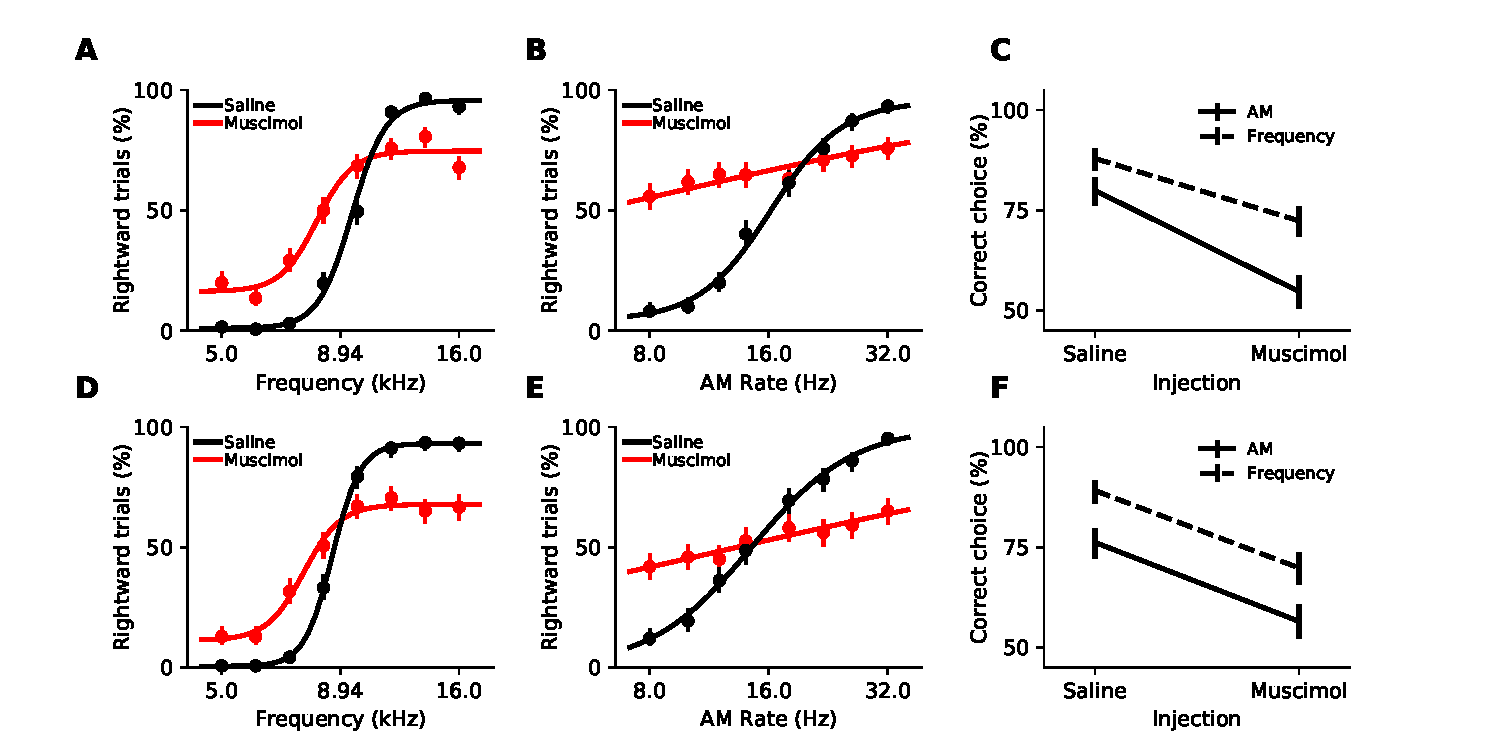
\includegraphics[width=6in]{figures/chapter4/figure_main_amod_effect}%
\end{center} \caption{Reversible inactivation of AC impairs both frequency and
AM discrimination.}{ \textbf{(A)} Frequency discrimination psychometric
performance for subject 1, averaged over 5 saline sessions (black points) and 5
muscimol sessions (red points).
%
\textbf{(B)} AM discrimination psychometric performance for subject 1, averaged
over 5 saline sessions (black points) and 5 muscimol sessions (red points). 
%
\textbf{(C)} Average percent correct for subject 1, averaged over 5 saline
sessions and 5 muscimol sessions.
%
Dotted line indicates the effect of muscimol injection on sound frequency
discrimination performance. 
%
Solid line indicates the effect of muscimol injection on AM rate discrimination
performance.
%
Error bars indicate 95\% binomial proportion confidence intervals.
%
\textbf{(D, E, F)} Same as A, B, and C, respectively, for subject 2.  }
\end{figure}
% 
% % The effect of inactivation is not different between the two stimuli (GLMER
% % results).
% 
% \subsection{AC inactivation affects discrimination of both features when during
% sessions with a single sound type}
% % DONE: Did they learn both, and then get transferred to 2? Was it the same
% % between?
% For a subset of animals, we performed reversible inactivation of AC during
% sessions where subjects only had to discriminate a single sound type.
% %
% Under these conditions, we still observed an effect of muscimol both on
% psychometric performance (\textbf{\fig{\SinglePsy}}) and on overall percent
% correct (\textbf{\fig{\SingleSum}}).
% 
% % We have a few sessions where we show that both discriminations are hurt
% % individually, arguing against the idea that the cortically-dependent part of
% % the task is the switching. 
% 
% %%%%%%%%%%%%%%%%%%%%%%%% Figure Single Sound Type %%%%%%%%%%%%%%%%%%%%%%%%%%%%%
% \begin{figure}[hp] \begin{center}
%     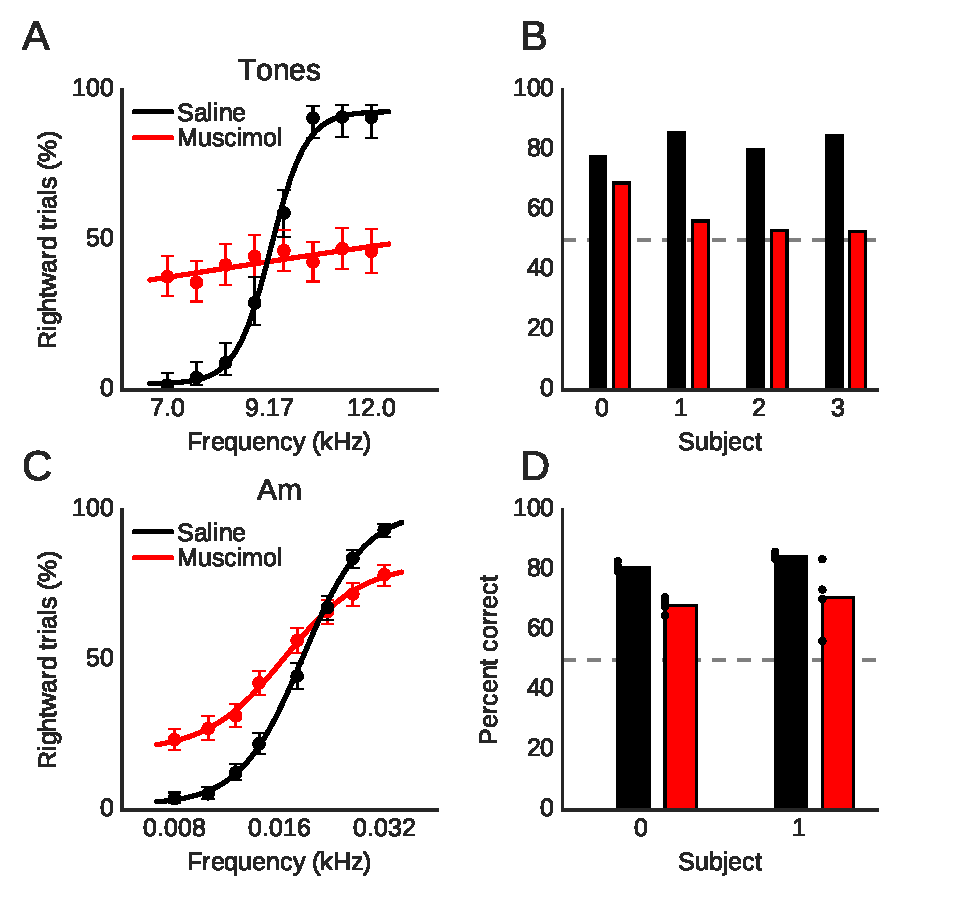
\includegraphics[width=6in]{figures/chapter4/figure_single_sound_type}%
% \end{center} \caption{Muscimol affects each discrimination when performed
% independently.}{\textbf{(A)}  Example psychometric curve from sessions where an
% animal discriminated only high sound frequency from low sound frequency.
% Performance suffers in sessions where muscimol was injected in AC (red, 1
% session) compared to control saline injection (black, 1 session).
% % DONE: How to have number of sessions here? 
% %
% \textbf{(B)} Average percent correct for 4 animals during muscimol (red, 1
% session per animal) and saline (black, 1 session per animal) sessions. 
% %
% \textbf{(C)} Example psychometric curve from sessions where an animal
% discriminated only fast AM rates from slow AM rates. Performance suffers in
% sessions where muscimol was injected in AC (red, 4 sessions) compared to
% control saline injection (black, 4 sessions).
% %
% \textbf{(D)} Average percent correct for 2 animals during muscimol (red, 4
% sessions per animal) and saline (black, 4 sessions per animal) sessions.  }
% \end{figure}


\section{Discussion}

This behavioral paradigm was designed to facilitate comparison of the same manipulation of neural activity on discrimination of two different sound features, in order to address the question: Is auditory cortex required for discrimination of some sound features, while discrimination of other sound features can be accomplished with subcortical pathways alone? 
%
We found that animals were able to learn the task, although it took a long time to train them to perform it at a high degree of accuracy. 
%
We performed reversible inactivation of auditory cortex in two animals trained in this task, and observed deficits in both frequency and AM discrimination. 
%
Future experiments must leverage the flexibility of the 2AFC paradigm, by manipulating the stimulus sets presented, to bring the psychometric performance for each sound type to the same starting point before performing inactivations. 
%
Importantly, we chose to use reversible inactivation with muscimol in this study for several reasons, but this behavioral paradigm can generalize to other inactivation techniques as well. 
%
It is likely that a full picture of the role of sensory cortex in the two discriminations tested would rely on information gained from inactivation experiments with different methods of manipulating or silencing activity. 

\subsection{Information from reversible inactivation vs. lesion experiments}
% What is the role of chemical inactivations when you could just do lesions so that you know the exact boundary of the removed tissue?
Lesions have the advantage of allowing precise histological determination of the regions that are removed or damaged. 
%
% NO : Refs
Lesions can also lead to different results than transient inactivations, an effect often assumed to be related to compensatory plasticity occurring after the lesion and before the behavioral assessment. 
%
However, the comparison of both lesion and transient inactivation experiments can lead to a fuller picture of the role of a brain area in a behavior. 
%
If a downstream region receives connections from both a cortical and a subcortical area, then transient inactivation of the cortical region could lead to unbalanced inputs in the downstream region and cause task deficits, even if the cortical representation of the information isn't any more useful for solving the behavioral task than the subcortical representations. 
%
Following a lesion of the cortical region, the downstream area could undergo homeostatic rebalancing of its inputs, and the discrimination could be solved again using only the input from the subcortical pathway. 
%
In this situation, the lesion study alone may lead to the erroneous conclusion that the cortical region is not at all involved in task performance under normal circumstances, and the transient inactivation experiment would lead to the erroneous conclusion that the information from the subcortical pathway is not sufficient, or at least less useful, for solving the discrimination task. 
%%%%%%%%

%%%%%%%%
A more nuanced way of examining the role of brain regions is laid out in \citet{Otchy2015}. 
%
The authors argue that brain areas should be categorized as \emph{necessary} or \emph{permissive} for task performance by using a combination of both lesion and transient inactivation experiments. 
%
An area is \emph{permissive} for task performance if it is involved in task performance under normal conditions, but doesn't provide any information that can't be obtained from other pathways or areas. 
%
Transient inactivation of a permissive structure will cause deficits in task performance, but lesion of the area, with a recovery period afterward to allow downstream areas to adapt to changes in their inputs, would not.
%
An area that is truly \emph{necessary} provides information that cannot be obtained from another source. 
%
Thus, performance would still suffer after lesion, even if you allow a period for downstream circuits to adapt.

% \subsection{What about using optogenetics instead?} % With opto you can use the same fiber over many sessions to standardize the location of the light delivery. 
% In the experiments presented here, we chose to perform transient inactivation using muscimol instead of using optogenetic methods. 
% %
% While optogenetic methods are unparalleled in their ability to allow circuit manipulations with fine temporal resolution, we preferred to use chemical inactivation in this case because we were interested in silencing cortex for the duration of the behavioral session. 

% NO: Do I want to finish this? 
% If you leave the light on you can burn the brain 
% Also, not all opsins can follow for long periods of time. 
% Most experiments use pulses of light to get around this, but this leads to the potential for local circuit interactions which can cause network activity to do unpredictable things. 

% 2. Fast time-scale manipulations can cause local network effects and mess with
% feedback inhibition and excitation, potentially messing everything up.
% %
% Chemical inactivations allow the brain area to reach a new steady-state that
% will persist for roughly the length of time that the animal is performing the
% behavior.
% %
% It might be possible to leave the light on if using cheeta or some other opsin
% that doesn't get weaker over time, but you run the risk of frying the brain.
% %
% Chemical inactivations don't have that issue. 

\subsection{What did we learn from preliminary inactivations?}
We performed inactivations over many behavioral sessions in two trained animals, showing that this method allows us to resolve the effect of the manipulations on discrimination of each sound type. 
%
However, interpretation was hampered by the fact that pre-inactivation performance was not equivalent between the two sound types. 
%
Therefore, it was not clear whether a decrease from 85\% correct to 75\% correct and decrease from 75\% correct to 65\% correct were effects of equivalent magnitude. 
% 
Future experiments should carefully match pre-inactivation performance between the sound types for each animal by adjusting the range of sounds presented during the psychometric sessions.
%
Nevertheless, it was clear from these inactivation experiments that there was an effect of cortical inactivation on discrimination of both sound types, and that evaluation of the relative necessity of sensory cortex for performing two discrimination of two different sound features will require precise comparison of the magnitude of the effect on each discrimination.

\section{Link to Chapter V}
In this chapter, we present a behavioral task for evaluating the effect of chemical inactivation of auditory cortex on frequency and AM rate discrimination performance. 
%
% DONE: Change this to highlight the results less. 
This behavioral paradigm provides a platform for evaluating the effect of a manipulation of neural activity on discrimination of two different stimuli, in order to address the question: Is the information provided by sensory cortex to downstream areas necessary for discrimination of some types of sounds, while discrimination of other sound types can be performed using information from subcortical pathways alone?
%
In the next chapter, we expand from considering just the role of auditory cortex in the context of this task, to examine the role of other sensory cortical regions in different tasks requiring animals to make flexible associations between stimuli and actions. 

 % Amod task
% Figures in this chapter
\newcommand{\Tasks}{5.1}
\newcommand{\StimOutcome}{\Tasks A}
\newcommand{\StimAction}{\Tasks B}
\newcommand{\FeatureRelevance}{\Tasks C}

\newcommand{\Mechanisms}{5.2}
\newcommand{\LTP}{\Tasks A}
\newcommand{\TopDown}{\Tasks A}

\chapter{The role of sensory cortex in behavioral flexibility}

\section{Journal style information}
\noindent Lan Guo, Nicholas D Ponvert, and Santiago Jaramillo. Reproduced in part from \textit{Neuroscience}, 2017. Copyright 2017.

\section{Author contributions}
Santaigo Jaramillo provided mentorship for all aspects of the study. Lan Guo, Nicholas D. Ponvert, and Santiago Jaramillo wrote the sections of the paper included in this dissertation.

%%%%% No abstracts inside chapters!
%% \section{Abstract}
%% To thrive in a changing environment, organisms evolved strategies for rapidly modifying their behavioral responses to sensory stimuli. In this review, we investigate the role of sensory cortical circuits in these flexible behaviors. 
%% %
%% First, we provide a framework for classifying tasks in which flexibility is required. We then present studies in animal models which demonstrate that responses of sensory cortical neurons depend on the expected outcome associated with a stimulus. Last, we discuss inactivation studies which indicate that sensory cortex facilitates behavioral flexibility, but is not always required for adapting to changes in environmental conditions.
%% %
%% This analysis provides insights into the contributions of cortical and subcortical sensory circuits to flexibility in behavior.

\section{Introduction}
Behavioral flexibility is defined as the ability to shift response patterns (or strategies) after changes in environmental conditions \citep{Ragozzino2007}. These environmental conditions define the statistical relations between a stimulus, possible behavioral responses, and outcomes (such as a rewards or punishments). We refer to these relations as \emph{contingencies}. 
%
The ability to adapt to changing contingencies is impaired in several human neurological disorders, including schizophrenia \citep{Goldberg1988,Morice1990} and autism \citep{Hill2004}. Our quest to develop better diagnostic and therapeutic strategies for these disorders would greatly benefit from detailed knowledge of the circuits and mechanisms responsible for flexibility in behavior.
%
Research on the neural basis of flexible behaviors in mammals has identified regions of the frontal cortex that detect changes in contingencies, inhibit undesired responses, and help acquire new strategies \citep{Dias1997,Ragozzino2007, Sotres-Bayon2010}. In contrast, it is not clear whether sensory cortex plays a role in implementing flexibility in behavior beyond extracting features of sensory stimuli. 

Understanding the neural mechanisms underlying flexible behaviors, and the role of sensory cortical neurons, requires monitoring neuronal activity with single cell resolution and manipulating the system in ways difficult to achieve in human subjects. For this reason, we focus here on experiments that use animal models of flexible behaviors.
%
We review studies in which sensory neurons are monitored or manipulated during changes in contingencies to address the following questions: What roles do sensory pathways play in behavioral flexibility beyond conveying sensory information? What flexible behaviors require sensory cortex? Which subcortical pathways can implement flexible behaviors without the need of the sensory cortex?

Several parallel neural pathways link sensation to action, including circuits in the brainstem that mediate reflexive responses, subcortical circuits via the amygdala that can mediate fear responses, and higher-order pathways that rely on sensory and motor cortex. In this review, we investigate how a stimulus can drive different behavioral responses depending on environmental conditions. A neuronal population within a sensory pathway can play at least three different roles during flexible behaviors. First, these neurons may be the first stage in the ascending sensory pathway that can discriminate the stimuli presented in a task. These neurons will be required for successful performance of the task, even though they do not play a direct role in rerouting information upon a contingency change. Second, this population may be the first stage in the ascending pathway that can communicate with circuits that reroute signals to implement behavioral flexibility. In this case, even though other regions (closer to the periphery) may be able to discriminate the stimuli in the task, information has to go through this specific stage before it can be flexibly rerouted to drive distinct actions.
% 
Third, a population of sensory neurons may play an active role in signal rerouting---passing or filtering out signals depending on the desired behavioral outputs for a given contingency. In this last scenario, we say that these neurons take part in implementing flexibility. 
%
Brain regions can play one or more of these roles, and do so in the context of coordinated activity across multiple other regions.

Here we review studies that quantify the correlations between sensory neural representations and behavioral contingencies. These studies indicate that sensory representations are modulated by expected outcomes associated with a stimulus, and when animals selectively attend to relevant stimulus features.
%
In addition, we discuss the behavioral effects of manipulating neural activity in sensory cortex during tasks that require flexibility. Sensory cortex lesions often impair behavioral adaptation following contingency changes. However, some flexible behaviors are possible after inactivation of sensory cortex.

\section{Taxonomy of adaptive behaviors}
%
In this section, we provide a framework for classifying different types of adaptive and flexible behaviors according to the relations between sensory stimuli, behavioral responses, and outcomes (such as rewards or punishments). We start by discussing phenomena in which these relations do not change, yet the nervous system can adapt to the statistics of a stimulus ensemble. We then discuss phenomena in which these relations do change, and classify these phenomena into three categories of flexible behaviors.

Neural correlates of adaptation to stimulus ensemble statistics can be observed even in anesthetized animals, and occur independently of reward contingencies. Examples include changes that result from contrast adaptation in the retina \citep{Baccus2002} and from adaptation to repetitive acoustic stimuli observed in the midbrain \citep{Malmierca2009}, thalamus \citep{Anderson2009} and cortex \citep{Ulanovsky2003}. 
%
In behaving animals, this adaptation provides a performance advantage by allocating neuronal resources to maximize the detection or discrimination of stimuli.
%
Some cases of \emph{perceptual learning}, defined as the improvement in sensory discrimination by practice \citep{Goldstone1998}, are examples of this type of adaptation without changes in reward contingencies. For instance, auditory cortical circuits change their sound frequency tuning as animals are trained to discriminate small differences in the frequency of sequentially presented tones \citep{Recanzone1993}.
%
In addition, subjects can use selective attention in tasks where the stimulus-action-outcome associations do not change.
In this case, subjects allocate resources to space \citep{Posner1980} or time \citep{Jaramillo2011} in order to improve task performance, resulting in changes of sensory cortical neural responses.
%
In all these scenarios, the relation between the stimulus, action and outcome does not change, and the only environmental feature driving adaptation is the stimulus ensemble. We exclude these phenomena from our discussion of behavioral flexibility. 

Here we focus on a different class of phenomena in which adaptation is driven by changes in the statistical relation between stimuli, behavioral responses and outcomes, \emph{i.e.}, changes in behavioral contingency. We first discuss scenarios in which the outcome associated with a stimulus varies across contingencies, as illustrated in \fig{\StimOutcome}. In this example, the star stimulus predicts a rewarding outcome in one condition (C1), but not in the other (C2). The circle stimulus, in contrast, is not associated with any outcome in the initial condition, but predicts reward when the contingency changes.
%
In this class of phenomena, which include acquisition and extinction of conditioned responses, actions may not be required to trigger a reward or punishment.

In the second type of scenario discussed, animals are required to change the action associated with a stimulus, but the outcome that can be achieved for each stimulus remains the same. 
%
This is illustrated with the discrimination task in \fig{\StimAction}. To obtain reward after a stimulus is presented, the subject must perform one of two possible actions: move right (R) or left (L). In the initial contingency (C1), the star stimulus predicts that the subject will obtain reward only after action R, while the circle predicts reward for action L. In contingency C2, the actions that yield reward for each stimulus are reversed. In contrast to the scenario described in \fig{\StimOutcome}, both stimuli predict reward under all contingencies in this task.
 
Separately, we discuss a special case of reversal phenomena in which selective attention can be used to filter out some features of the stimulus (\fig{\FeatureRelevance}).
%
During stimulus-driven behaviors, not all features of the environment are relevant at all times, \emph{i.e.}, some features may not predict outcomes. Depending on how the relevance of stimulus features changes across contingencies, we can define two different types of tasks. In the reversal task presented in \fig{\StimAction}, irrelevant features of the stimulus (such as the background in which it is presented) never become relevant. In contrast, parts of the stimulus in the task presented in \fig{\FeatureRelevance} change from being predictive of reward to being irrelevant. In this scenario, it can be advantageous for the organism to filter out a different set of irrelevant features in each contingency by engaging selective attention. The right panel of \fig{\FeatureRelevance} illustrates the advantage provided by attention. In a task defined by a contingency table with 16 entries (8 for each of the two contingencies), an animal would need to learn all possible combinations to maximize performance. Alternatively, the animal could learn that under each contingency, only half of the stimulus is predictive of reward. Thus, if the animal can filter out the irrelevant half of the stimulus under each condition, only 4 entries must be learned to successfully perform the task. In the next sections, we review studies that monitor or manipulate sensory representations during these three types of flexible behaviors.

%%%%%%%%%%%%%%%%%%%%%%%% Figure Tasks %%%%%%%%%%%%%%%%%%%%%%%%%%%%%
\begin{figure}[hp]
  \begin{center}
    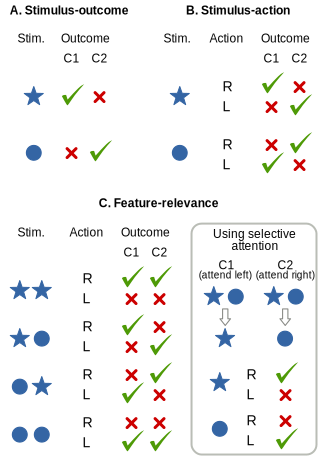
\includegraphics[height=5in]{figures/chapter5/figure_tasks}% 
  \end{center}
\caption{Types of flexible behaviors.}{Each panel shows the contingency table for a different type of task. The presence of an outcome, such as a reward, is indicated with a green check mark. A red cross mark indicates no outcome. (A) A task in which each stimulus (Stim.), either a star or a circle, presented in isolation predicts reward during one contingency (C1 or C2) but not the other. (B) A reversal task in which the possible outcomes for each stimulus remains the same, but the action, right (R) or left (L), required to obtain each outcome changes across contingencies. (C) A task in which a pair of items is presented simultaneously, but only one location is predictive of reward in each contingency. Animals can solve this task either by learning the full contingency table (left) or by using selective attention to filter out irrelevant regions/features of the stimulus (right box top) and applying a simpler contingency table for individual items (right box bottom). 
}
\end{figure}
%%%%%%%%%%%%%%%%%%%%%%%%%%%%%%%%%%%%%%%%%%%%%%%%%%%%%%%%%%%%%%%%%%%%%


\section{Stimulus representations in sensory cortex are modulated during flexible behaviors}

Do the responses of neurons in sensory pathways change depending on behavioral contingency? 
%
To address this question, we review studies that examine the neural representations of sensory stimuli before and after changes in stimulus-outcome associations (as in \fig{\StimOutcome}), stimulus-action associations (\fig{\StimAction}), and during flexible tasks in which animals can use selective attention to increase performance (\fig{\FeatureRelevance}).
%
We first present evidence that neural responses in stages as early as the sensory midbrain are influenced by the outcome associated with a stimulus.
%
These modulatory effects are present in a smaller percentage of sensory neurons if animals are required to modify their behavior in response to a stimulus, but the amount of reward (or punishment) associated with the stimulus remains the same.
%	
Last, we show that in tasks where features of the stimulus change relevance under different contingencies, attentional processes can strongly modulate sensory representations.

\subsection{Stimulus-outcome associations affect sensory representations}

Manipulation of stimulus-outcome associations can be achieved in the laboratory via several procedures including classical conditioning and extinction of conditioned responses. In classical conditioning, presentation of a conditioned stimulus (CS) is followed by either a punishment or a reward. Animals learn to associate this previously neutral stimulus with the outcome such that after conditioning the CS itself can elicit a conditioned response. This type of learning strongly modulates stimulus-evoked neural activity in sensory pathways. For instance, in the auditory system, these effects are evident in the midbrain, the medial division of the medial geniculate nucleus of the thalamus (MGm), primary auditory cortex (A1) and secondary auditory cortex (A2) \citep[reviewed in][]{Weinberger1987, Weinberger1993}, with sensory cortex neurons displaying longer-lasting modulation than midbrain and thalamic neurons \citep{Suga2003, Weinberger2007}. The firing rate of a large fraction of sound-responsive neurons in the MGm (71\% of cells), A1 (63\%), and A2 (95\%) is significantly modulated by the acquisition of a stimulus-outcome association in the cat \citep{Ryugo1978, Weinberger1984, Diamond1984}. In these experiments, MGm neurons showed 20-30\% changes in firing rate, whereas larger firing rate changes were observed in the cortex: 200-300\% change in A1 and 50-150\% in A2 \citep{Ryugo1978, Weinberger1984, Diamond1984}. In addition to changes in the size of evoked responses, altering stimulus-outcome associations modulates the receptive field properties of up to 75\% of auditory cortical neurons \citep{Fritz2003} and up to 60\% of inferior colliculus neurons in ferrets \citep{Slee2015}. 

Conditioning-induced increases in evoked neural activity are reversed during extinction of conditioned responses, \emph{i.e.}, when repeated presentation of the CS without reinforcement results in a decrease in the conditioned response.
In one study, auditory- and visual-responsive neurons in posterior thalamic nuclei that project to the amygdala and striatum in addition to sensory cortex showed responses to CS predictive of reward, with response amplitude proportional to the reward size \citep{Komura2001}. The sensory responses in these thalamic neurons decreased in amplitude or disappeared during extinction of the stimulus-reward association, and responses were again potentiated during reinstatement of reward. Separate studies showed that enhanced neuronal responses to a CS in the auditory cortex and the thalamus were reduced when the CS no longer predicted outcome \citep{Gabriel1976, Edeline1990}. 
Moreover, the area of auditory cortex responsive to the CS expands following conditioning and contracts following extinction, and the degree of contraction is correlated with the strength of extinction measured behaviorally \citep{Bieszczad2012}.
Overall, studies using conditioning acquisition and extinction reveal that stimulus-outcome associations modulate responses in sensory structures from midbrain to cortex in a reversible manner.

\subsection{Stimulus-action associations influence only a minority of sensory neurons}

In a different set of studies, the action required to obtain reward (given a stimulus) changed, but the amount of reward remained the same.
%
For example, a rhesus monkey was trained to perform an auditory discrimination task where a tone or a noise stimulus required shifting a lever left or right, respectively, to obtain reward. The stimulus-action contingency was then reversed, while the sound-evoked responses from the auditory cortex were measured. Although the majority of single-units recorded in the auditory cortex showed sensory-evoked responses, only 17\% of the sensory-responsive neurons showed responses modulated by the stimulus-action contingency \citep{Vaadia1982}. A separate study in rats found a similar modulation of evoked responses from both cortical and thalamic auditory neurons \citep{Jaramillo2014a}. Animals were trained to categorize sounds as low- or high-frequency by choosing the left or right reward ports of a training chamber after the presentation of a stimulus \citep{Jaramillo2014b}. The categorization boundary that separated low- from high-frequency sounds was shifted several times within each behavioral session, requiring animals to change the action associated with some stimuli. In this task, the reward given for a correct response was always kept constant. Therefore, the stimulus-outcome association remained the same throughout the task, while the stimulus-action association changed from one block of trials to the next. Only 15\% of responsive auditory cortical neuronsc and 16\% of responsive thalamic neurons were modulated by changes in the stimulus-action association. 
%
These studies suggest that a smaller percentage of neurons in sensory cortex and thalamus are modulated by changes in the behavioral response associated with a stimulus than by changes in the magnitude of reward. It is still possible that such a small percentage of cells can have an effect on behavior.

\subsection{Selective attention modulates sensory representations}

In some scenarios, subsets of features of a sensory stimulus that are initially relevant in predicting an outcome can become irrelevant. Subjects could solve these tasks by learning all relations between stimuli, actions and outcomes. A more efficient strategy requires using selective attention to filter out irrelevant features without the need for changing the associations between stimulus, actions and outcomes (\fig{\FeatureRelevance}).

The effects of attention on neuronal responses have been reviewed extensively \citep{Treue2001, Maunsell2002, Reynolds2004}. If two stimuli are presented within the receptive field of a neuron in the visual cortex, directing attention to one or the other stimulus strongly modulates the evoked activity in a large percentage of neurons. In area V4 of primates, 40-80\% of neurons display significant modulation of stimulus-evoked responses due to attention \citep{Motter1993, Luck1997, Reynolds1999, McAdams1999}, resulting in a 40-65\% change in firing rates \citep{Luck1997, McAdams1999}. Similar experiments show that roughly 80\% of cells in areas MT and MST are significantly modulated by attention, with a median firing rate modulation magnitude of about 80\% for MT and 100\% for MST \citep{Treue1996, Treue1999}. When two competing stimuli are far enough apart that they do not fall within the receptive field of a single neuron, the effects of attention are smaller, with only 13\% of V4 neurons displaying significant modulation \citep{Luck1997}. Roughly 50\% of neurons in areas MT and MST are modulated by attention under these conditions, with a median firing rate modulation of 19\% in MT and 40\% in MST \citep{Treue1996}. In addition to focusing attention on specific areas of visual space, subjects can direct attention to specific attributes of a stimulus. This type of feature-based attention also modulates the responses of visual cortex neurons \citep[reviewed in][]{Maunsell2006}. For instance, when monkeys were required to report the orientation of the stimulus that matched a color cue (and ignore all other stimuli), 74\% of V4 neurons displayed higher firing rate when the stimulus inside their receptive field matched the cued color compared to when a different color was cued. This effect of attention resulted in a doubling of the stimulus-evoked firing rate in these neurons \citep{Motter1994a}.

The effects of both spatial and feature-based attention have also been studied in the auditory system \citep{Fritz2007b, Hromadka2007}, although to a lesser extent. In an auditory-visual cross-modal attention task, roughly 67\% of stimulus-responsive neurons in the auditory cortex showed activity modulated by whether the monkey was required to respond to the light or respond to the sound \citep{Hocherman1976}. In human fMRI studies of multimodal attention, attending to one modality increased the response in the sensory cortical region corresponding to the attended modality and decreased activity in the sensory cortical region corresponding to the unattended modality \citep{Johnson2005}. Overall, these studies show that shifting attention largely modulates neuronal responses in sensory cortex.

\subsection{Summary of changes in sensory representations during flexible behaviors}
The studies reviewed in this section demonstrate that sensory neurons can integrate and represent stimulus relevance. Stimulus-evoked responses in over half of the recorded sensory neurons from areas in the midbrain to the cortex are modulated by changes in the outcome associated with a stimulus. This stimulus-outcome modulation is reversible on the same time scales as the behavioral changes. Moreover, changes in the relevance of stimulus features can engage attentional processes and result in modulation of sensory responses. In comparison, changing the action associated with a stimulus without changing the associated outcome yields modulation of responses in less than a fifth of neurons in sensory cortex and thalamus.

\section{Is sensory cortex required for behavioral flexibility?}

Correlational studies can reveal the environmental features that are represented in a brain region. However, manipulation studies are needed to provide information about the causal relationship between brain activity and behavior. 
Studies that inactivate sensory cortex find a wide range of effects on detection and discrimination of stimuli in audition \citep{Talwar2001, Rybalko2010, Gimenez2015, Kato2015} and vision \citep{Birch1978, Oakley1981, Glickfeld2013}. The largest effects are often seen for the discrimination of complex stimulus features, \emph{i.e.}, those not represented explicitly in the periphery \citep{Newsome1988, Ohl1999, Deutscher2006}. It is well established that selectivity for stimulus features of higher complexity increases in the ascending sensory pathways from the periphery to cortical regions \citep{Hubel1962, Miller2001a, Joris2004}.
%
When complex stimuli are used in a task, cortical lesion impairs discrimination performance, which makes it difficult to differentiate whether the cortex plays a role in implementing flexibility or simply transfers information to downstream structures that implement flexibility. Although animals are often exposed to stimuli of high complexity in their natural environments, experimental manipulations in the laboratory often use well-controlled simple stimuli in order to tease apart functional roles in stimulus processing versus roles in mediating flexible behavior.

\subsection{Sensory cortex facilitates extinction of stimulus-outcome associations} 


Studies that used aspiration or electrolytic lesions of sensory cortices before fear conditioning have found that acquisition of the conditioned fear response can still occur in the auditory \citep{Teich1989, Campeau1995, Song2010} and visual domains \citep{LeDoux1989, Falls1993}. 
%
Similarly, post-training excitotoxic lesions of the primary auditory cortex did not attenuate fear-potentiated startle in rats after 10 days of recovery \citep{Campeau1995}. 
%
However, more extensive post-training electrolytic lesions spanning secondary auditory and perirhinal cortex blocked fear memory recall, at least for the periods tested \citep{Campeau1995, Boatman2006}. Additional evidence of a cortical role in associative learning comes from a study in which protein synthesis inhibitors were applied to the auditory cortex during conditioning to frequency-modulated sounds \citep{Kraus2002}. 
%
This manipulation impaired the speed of learning, although application of the inhibitors in well-trained animals did not impair recall of the conditioned behavior. 

The effects of sensory cortex lesions on the extinction of conditioned responses have also been inconsistent across studies \citep[reviewed in][]{Myers2002}. 
%
For example, one study found that complete aspiration lesions of the visual cortex 10 days before fear conditioning to a visual CS did not prevent subsequent extinction \citep{Falls1993}. Other studies that also used pre-acquisition lesions of sensory cortex found impairments ranging from a slowdown of extinction \citep{Song2010} to a complete inability to extinguish the conditioned response for the periods tested \citep{LeDoux1989, Teich1989}.
%
Under some task conditions, pre-acquisition lesions of auditory cortex can severely impair the ability to respond flexibly to changing sound-outcome associations \citep{Ono2006}.
%
In these conditions, it appears that the impairment was not in the extinction of acquired associations, but either in the ability to form new associations or to respond to only the rewarded stimulus.
%
Post-acquisition lesions of sensory cortex have also been shown to retard responses to changing stimulus-outcome associations. For example, when rats were trained to associate an increase in stimulus intensity (the CS) with a footshock, sensory cortex lesions after acquisition resulted in slower adaptation when the CS was changed to a decrease in stimulus intensity. These effects were observed in both the auditory and visual domains \citep{Delay1994}. 


If fear conditioning can still proceed in the absence of sensory cortex, what subcortical sensory pathways mediate this behavior? Inactivation studies have found that both thalamo-amygdala and cortico-amygdala pathways can transfer information about an auditory conditioned stimulus during fear learning \citep{Romanski1992, Campeau1995}. Involvement of the thalamo-amygdala connections in conditioning is also supported by observations of conditioning-induced plasticity in these synapses \citep{McKernan1997, Quirk1997, Maren2004}. Altogether, these results suggest that multiple parallel pathways are engaged in fear conditioning in the intact brain.


\subsection{Sensory cortex is not always required for reversal learning of stimulus-action associations}

The role of sensory cortex in reversal learning has been investigated by treating the auditory cortex of gerbils with enzymes that degrade the extracellular matrix \citep{Happel2014}. This procedure, which restores juvenile-like levels of plasticity \citep{Pizzorusso2002, Gogolla2009}, made animals faster at reversing the action associated with frequency-modulated sounds. These results suggest a causal role of cortical plasticity in the reversals of stimulus-action associations. 
%
Other studies, however, show that animals can perform reversals of stimulus-action associations after extensive lesions of sensory cortex.

A study in rats tested performance on a visual discrimination task 12-25 weeks after near complete ($>$95\%) removal of the entire neocortex.
%
Animals discriminated between a door that was marked with a horizontal grating and a door marked with a vertical grating, one of which signaled the presence of a food reward. Lesioned animals were only slightly slower than controls at learning this behavior. When the pattern that signaled the correct door was reversed, lesioned animals took longer than controls to learn the reversal but were eventually able to reach the same performance criterion (18 correct choices in a row) as control animals \citep{Oakley1981}.
%
Another study using a similar visual discrimination paradigm found that rats with posterior decortication six weeks before training were also slower at reversing learned associations than controls \citep{Birch1978}. In this study, lesioned rats were less impaired when they only had access to light intensity cues, compared to when they were exposed to all spatio-visual cues, suggesting that cortical involvement in reversal learning depends on stimulus complexity. 


In the studies presented above, animals received lesions before behavioral training. A recent study investigated the effects of lesions after animals had been extensively trained to perform a flexible sound categorization task \citep{Gimenez2015}. In this task, animals must reverse the action associated with a sound multiple times over the course of a single session.
%
Rats were able to switch the action associated with a spectrally-simple sound to obtain water reward, even on the first post-lesion session that tested reversals (3-5 days after the surgery). The number of trials to switch was comparable before and after lesion. 
%
In contrast, lesions of the auditory thalamus severely impaired the ability to discriminate sound frequencies in this task, therefore preventing the expression of the flexible categorization behavior. All together, these results suggest that subcortical outputs of the auditory thalamus are capable of mediating this behavior.

Compensatory plasticity in subcortical circuits could explain why animals in these studies were able to perform reversal learning after cortical lesions.
%
However, when well-trained rats were tested during reversible bilateral inactivations of auditory cortex using muscimol, they were still able to flexibly switch between the previously-learned sound-action associations \citep{Gimenez2015}. These results suggest that if compensatory mechanisms are involved, they may be fast-acting. 
%
Overall, sensory cortex does not always appear to be required for flexible tasks where the action associated with a stimulus must be modified.
\subsection{Ability to filter out distractors is impaired by lesions of sensory cortex}  

Evidence that areas of the visual cortex are necessary for shifting attention comes mostly from studies that evaluate the effect of distractors on visual perception in primates before and after lesions. For instance, aspiration lesions of area V4 after extensive behavioral training largely affected the ability to saccade to a target item immersed in an array of other similar items \citep{Schiller1991}, although the ability to detect this stimulus in isolation was minimally affected. Similarly, aspiration lesions of areas V4 and TEO impaired the animals' ability to detect changes in the orientation of a stimulus when surrounded by high-contrast distractors \citep{DeWeerd1999}. The effect was minimal when the stimulus was presented in isolation. These effects were replicated for detection of color changes, but were not present during detection of changes in motion \citep{DeWeerd2003}. Because neurons in areas V4 and TEO are highly selective to orientation and color, but less so to motion, these results imply that the ability to ignore distracting visual features depends on the neural substrate that processes the relevant feature in a given task. 
Impaired ability to filter out visual distractors has also been observed in human patients with brain damage to the temporal lobe \citep{Mendola1999} and at the temporal-occipital junction \citep{Gallant2000}.

Studies of cortical lesions in humans also suggest impairments in spatial attention during dichotic listening tasks \citep{Woods1993, Bellmann2001}. However, since lesions are not always restricted to the auditory cortex, the exact cause of behavioral deficits are difficult to determine. 

\subsection{What have we learned from lesion studies?}
The studies reviewed in this section provide insights into the possible roles played by the sensory cortex during flexible behavior, and help determine what subcortical sensory pathways can do in the absence of the cortex.
% 
In the intact brain, sensorimotor selection likely involves coordinated activity in multiple regions, such that inactivating any of these could lead to an impairment \citep{Du2011}. The studies reviewed here indicate that sensory cortex lesions slow down the extinction of learned stimulus-outcome associations, as well as the reversal of stimulus-action associations, but do not always preclude these behaviors. Sensory cortex seems to be essential for filtering out distractors during attention tasks. 

Negative results from cortical lesion studies cannot rule out cortical involvement in a given behavioral task. The existence of multiple parallel pathways, or the reorganization of sensory circuits (compensatory plasticity), are potential explanations for the ability to perform flexible behaviors after cortical lesions. Compensatory plasticity can come about either through the formation of new pathways or through adaptation of downstream areas to changes in their inputs. An example of compensatory plasticity can be seen from studies of amplitude-modulated (AM) sound discrimination. Serial lesions of bilateral auditory cortices in Mongolian gerbils with intervening training did not result in an impairment on discrimination performance for fast AM tones \citep{Depner2014}. In contrast, simultaneous bilateral ablations led to complete loss of AM discrimination in the same paradigm \citep{Deutscher2006}. Training after the first unilateral lesion potentially triggers compensatory plasticity in subcortical pathways, which could compensate for the loss of cortical function. 

The development of new tools to manipulate neuronal activity has made possible the transient inactivation of neuronal circuits on a millisecond time scale. Such acute inactivation can potentially diminish the confounding effects of compensatory plasticity. However, if we wish to know whether brain regions besides the sensory cortex have the capabilities necessary for mediating a behavioral task, long-lasting cortical inactivations may still be advantageous. Acute inactivation can lead to sudden perturbations of information in downstream structures. Due to this transient imbalance in the circuit, acute inactivation experiments could potentially overestimate the functions carried out by the affected cortex, and make it difficult to test the sufficiency of subcortical areas alone \citep{Otchy2015}.

\section{Conclusions and future directions}
This review set out to address the role of sensory cortex in flexible behavior and what subcortical pathways can do in the absence of the cortex.
%
In summary, changing the expected outcome associated with a stimulus largely modulates sensory representations. Under these conditions, cortical inactivation affects the extinction of these stimulus-outcome associations without disrupting the acquisition.
%
In comparison, a smaller percentage of sensory neurons are modulated when behavioral responses must change in response to a stimulus, but the outcome associated with the stimulus remains the same. In this case, lesions of sensory cortex either slow down or do not affect the ability to update stimulus-action associations.
%
In tasks where selective attention can be used to filter out irrelevant stimuli, sensory cortex lesions lead to impaired performance, consistent with the large modulation of cortical neuronal activity observed during these tasks.
%
These results will guide future investigation of selection mechanisms in neuronal pathways that link sensation to action. 

Flexibility in behavior can be implemented either by selection of stimuli or by selection of actions, via two (and possibly more) distinct neural mechanisms. First, feedback about outcomes can result in long-term changes in synaptic strength along the sensorimotor pathway, such that a stimulus is linked to its appropriate response under each contingency (\fig{\LTP}). Such long-term changes can be observed in the synaptic strength in brain slices from trained animals \citep{McKernan1997, Xiong2015}. Second, neural signals from outside the sensorimotor pathway can influence which sensory signals drive particular actions, without the need of synaptic changes in this pathway (\fig{\TopDown}). This mechanism has been shown to account for attentional modulation of neural activity \citep{Jaramillo2007}. 
%
It is possible that neural circuits employ both of these selection mechanisms in parallel to implement behavioral flexibility.

%%%%%%%%%%%%%%%%%%%%%%%% Figure Mechanisms %%%%%%%%%%%%%%%%%%%%%%%%%%%%%
\begin{figure}[hp]
  \begin{center}
    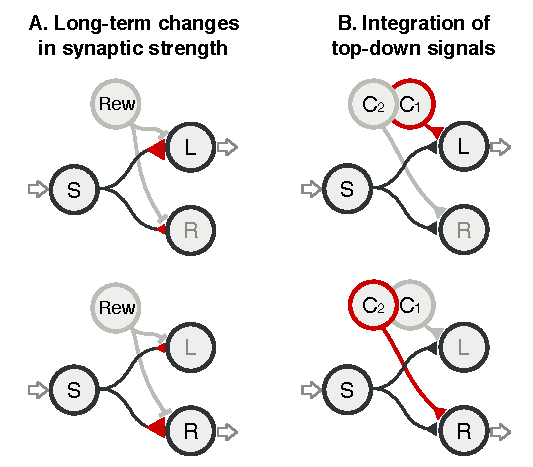
\includegraphics[height=4in]{figures/chapter5/figure_mechanisms}% 
  \end{center}
\caption{Two possible neuronal mechanisms for signal selection.}{Red indicates what changes in each scenario. (A) Signals from a sensory neuron (S) can be routed to drive different action neurons (R or L) by changing the synaptic strength of each pathway according to previous outcomes. In this scenario, reward-related signals (Rew) enable synaptic plasticity driven by the activity of pre- and post-synaptic neurons. The same sensory signal will drive action L (top) or R (bottom) depending on contingency. (B) Signals can also be routed without changes in synaptic strength in the sensorimotor pathway. In this scenario, top-down neurons that are selectively active in each contingency (C1 and C2) will bias which of the actions will be selected in response to sensory inputs. 
}
\end{figure}
%%%%%%%%%%%%%%%%%%%%%%%%%%%%%%%%%%%%%%%%%%%%%%%%%%%%%%%%%%%%%%%%%%%%%


How can we test which selection mechanism is recruited in the cortex during tasks that require behavioral flexibility? A first approach requires manipulating synaptic strength in competing sensorimotor pathways to test whether encoding of stimulus-outcome or stimulus-action associations is affected. For instance, induction of long-term potentiation and depression in cortico-amygdala and thalamo-amygdala synapses is sufficient to recapitulate the stimulus-outcome associations that result from classical conditioning \citep{Nabavi2014}. Similarly, manipulating potential sources of top-down signals can be used to test whether these signals are sufficient to drive sensorimotor selection, as has been done during visual selective attention \citep{Moore2003, Moore2004}. Lastly, blockade of plastic synaptic changes in sensorimotor pathways (without affecting synaptic transmission) can be used to test whether these changes are necessary for encoding stimulus-outcome associations \citep{Kraus2002, Quirk2008, Johansen2014}.
%
Using these tools, future studies can tease apart the conditions under which each of these two mechanisms is at play in sensory cortices. 
%
Impairments in behavioral flexibility observed in some neurological disorders \citep{Goldberg1988,Morice1990,Hill2004} could be the result of abnormalities in the components that regulate either of these selection mechanisms.  
%
Detailed knowledge of these mechanisms will inform development of effective treatment strategies for these disorders.


 % Subcortical flexibility
\chapter{Conclusion}

The experiments in Chapter 2 indicated a crucial role for the posterior striatum during performance of an auditory discrimination task. 
%
Previous literature had suggested a role for the pathway between auditory cortex and the posterior striatum in the context of a similar auditory task, which is consistent with the results of the inactivation experiments.
%
However, a model in which the corticostriatal pathway is solely responsible for facilitating behaviors involving discriminations of sound frequency are not consistent with lesion studies, which show that animals have a remarkable ability to perform auditory decision-making tasks, even requiring rapid flexibility, without auditory cortex. 
%
We therefore investigated the relationship between the auditory corticostriatal pathway and the parallel thalamostriatal pathway, interested in how these two sources of auditory input to the striatum compare and how they contribute to auditory decision-making tasks under different conditions. 

We found that the thalamostriatal and corticostriatal pathways convey information about sound frequency to the striatum with similar fidelity, potentially explaining why animals were found to be able to perform frequency discrimination tasks without auditory cortex. 
%
We also found that the representation of other sound features differed. 
%
Specifically, we found that the corticostriatal and thalamostriatal pathways differed in their representation of AM rate, with corticostriatal neurons more likely to be tuned to particular AM rates, and less likely than thalamostriatal neurons to synchronize their firing to the envelope of the modulation.
%
% TODO: Cite Deutscher, whatever else.
Based on these observations, and studies which suggested that AM discrimination performance suffers after auditory cortical lesion, we hypothesized that this cortical representation of AM rate better allows downstream circuits to perform discrimination of AM rate.

To test this hypothesis, we designed a task to compare the effect of a cortical manipulation on both AM rate discrimination and frequency discrimination in the same behavior session. 
%
Although it was difficult for animals to learn this task, with sufficient training they were able to achieve high levels of performance on both discrimination tasks. 
%
Pilot inactivation studies in animals performing this task suggested that AC inactivation impairs both frequency and AM rate discrimination behavior, and allowed us to identify key areas for future improvement of this method that would better enable comparisons of the magnitude of the effect on the performance of each discrimination. 
%
Principally, future experiments should better leverage the flexibility of the two-alternative forced-choice paradigm by changing the stimulus sets in order to make each discrimination easier or harder, allowing better matching of pre-inactivation performance between the two modalities.
%



%I found that inactivation of posterior striatum causes task deficits, and that these task deficits can't easily be explained by motor deficits alone.
%
%This is consistent with the other experiments in the paper, which showed that activation of posterior striatal neurons does not directly cause head rotation but does cause behavioral biases if done while the animal is performing a task. 
%
%The results of this inactivation are also largely consistent with the results of \citet{Znamenskiy2015}, in that they point to a key role for the auditory striatum in the performance of frequency-discrimination tasks. 


%Striatal activation, in our hands, resulted in strong contralateral biases regardless of the preferred frequency of the striatal neurons. 

% TODO: Check supplemental of ref 10 in Lan's paper (I think Petr). 
Zador lab stimulated AC without frequency-specific and found a contralateral bias.

Both of these pieces of evidence point towards the MSNs in the pStr acting as drivers of contralateral choice. 

% Do we see these ``contralateral'' biases only because we are using a left/right task? What about a go/no-go task? 

How can behavioral and neurophysiological comparisons help reveal the role of a brain area?

If an area is directly making the decision, then the responses of neurons there should be different when animals make a different choice but the presented sounds are the same. 

Can test whether the pre-withdrawal activity encodes an animal's choice.

Both of these have the choice being variable because the stimulus is close to the categorization boundary. So you can also do reversal tasks where the stimulus-action association is clear but changes between contingencies. 

%%%% Stuff related to Thstr paper

% What evidence exists for synaptic plasticity at thalamostriatal synapses?
% Look at thalamoamygdala
It is not known whether connections between sensory thalamus neurons and neurons in the striatum are capable of the same type of learning-related plasticity observed in corticostriatal synapses \citep{Xiong2015}, although plasticity has been observed between intralaminar thalamus and striatum \citep{Parker2016}.
%
One study has shown that simultaneous stimulation of auditory corticostriatal and thalamostriatal neurons leads to long term potentiation at corticostriatal synapses but not at thalamostriatal synapses, suggesting that, if the thalamostriatal pathway is capable of synaptic plasticity, different rules may govern the changes. 
% TODO: I am here
Plasticity does occur between neurons in the thalamus and those in the amygdala following fear conditioning,
cocaine conditioning \citep{Rich2019}

% The recording experiments happened in untrained animals. What might happen if animals are trained before? Where would the changes potentially occur? 

% Do thalamostriatal and corticostriatal inputs converge on the same MSNs?

% What does it mean for the inputs onto MSNs if the MSNs in posterior striatum may not be the ones actually performing the selection? 

% TODO: Check out Brice B's paper showing that for simple stimuli the thalamic pathway takes over, but for complex stimuli the reaction times are longer and the cortical pathway seems required. 


% Might cortex just be serving to reduce complex stimuli to simple rate-tuned representations? 

%%%%%%%%%%%%% Structure %%%%%%%%%%%%%%%%%
% Cortico-striatal involved, but on a similar task cortex is not necessary once animal has learned. We showed that striatum is required for task performance.
% We then turned to the thalamostriatal pathway, and compared the sound information being sent via that pathway and the corticostriatal pathway. Freq same, AM different.
% This raises the question of whether the thalamostriatal pathway is sufficient for the performance of some kinds of tasks, but not sufficient for others. A review of the literature related to the role of cortex in behavioral flexibility supports this idea.
% We designed and implemented a behavioral task that would allow the effect of a manipulation (such as chemical inactivation of AC) on performance of two discrimination tasks, frequency and AM rate.

% Overall in this dissertation we found:
%% Striatum is for sure a part of the system for performing sound frequency discriminaton discrimination behavior
%
%% The thalamostriatal and corticostriatal pathways send complementary information about sounds, but it isn't super clear why.
%
%% A review of the role of cortex in flexible behavior suggests that there are some classes of behaviors that can be performed without cortex, but there are some classes of beahviors where cortex is necessary.
%
%% We developed a task that can be used to evaluate the side-by-side effects on discrimination of different sound features.
%

 % Conclusion

\bibliographystyle{jneurosci}
\bibliography{/home/nick/library/Dissertation}%%uses BibTex formatting.

\end{document}
